%============================================================================
% tento soubor pouzijte jako zaklad
% (c) 2008 Michal Bidlo
% E-mail: bidlom AT fit vutbr cz
%============================================================================
% kodovaní: iso-8859-2 (zmena prikazem iconv, recode nebo cstocs)
%----------------------------------------------------------------------------
% zpracování: make, make pdf, make desky, make clean
% pøipomínky posílejte na e-mail: bidlom AT fit.vutbr.cz
% vim: set syntax=tex encoding=latin2:
%============================================================================
\documentclass[cover]{fitthesis} % odevzdani do wisu - odkazy, na ktere se da klikat
%\documentclass[cover,print]{fitthesis} % pro tisk - na odkazy se neda klikat
%\documentclass[english,print]{fitthesis} % pro tisk - na odkazy se neda klikat
%      \documentclass[english]{fitthesis}
% * Je-li prace psana v anglickem jazyce, je zapotrebi u tridy pouzit 
%   parametr english nasledovne:
%      \documentclass[english]{fitthesis}
% * Neprejete-li si vysazet na prvni strane dokumentu desky, zruste 
%   parametr cover

% zde zvolime kodovani, ve kterem je napsan text prace
% "latin2" pro iso8859-2 nebo "cp1250" pro windows-1250, "utf8" pro "utf-8"
%\usepackage{ucs}
\usepackage[utf8]{inputenc}
\usepackage[T1]{fontenc}
\usepackage{url}
\DeclareUrlCommand\url{\def\UrlLeft{<}\def\UrlRight{>} \urlstyle{tt}}

%zde muzeme vlozit vlastni balicky


% =======================================================================
% balíèek "hyperref" vytváøí klikací odkazy v pdf, pokud tedy pou¾ijeme pdflatex
% problém je, ¾e balíèek hyperref musí být uveden jako poslední, tak¾e nemù¾e
% být v ¹ablonì
\ifWis
\ifx\pdfoutput\undefined % nejedeme pod pdflatexem
\else
  \usepackage{geometry}
  \usepackage{listings}
  \usepackage{color}
  \usepackage[usenames,dvipsnames,svgnames,table]{xcolor}
  \usepackage[unicode,colorlinks,hyperindex,plainpages=false,pdftex]{hyperref}
  \definecolor{links}{rgb}{0.4,0.5,0}
  \definecolor{anchors}{rgb}{1,0,0}
  \def\AnchorColor{anchors}
  \def\LinkColor{links}
  \def\pdfBorderAttrs{/Border [0 0 0] }  % bez okrajù kolem odkazù
  \pdfcompresslevel=9
\fi
\fi

%Informace o praci/projektu
%---------------------------------------------------------------------------
\projectinfo{
  %Prace
  project=BP,            %typ prace BP/SP/DP/DR
  year=2014,             %rok
  date=\today,           %datum odevzdani
  %Nazev prace
  title.cs={Systém monitorování stavu plánovacích úloh},  %nazev prace v cestine
  title.en={Planning Task Monitoring System}, %nazev prace v anglictine
  %Autor
  author={Martin Maga},   %jmeno prijmeni autora
  %author.title.p=Bc., %titul pred jmenem (nepovinne)
  %author.title.a=PhD, %titul za jmenem (nepovinne)
  %Ustav
  department=VCIT, % doplnte prislusnou zkratku: UPSY/UIFS/UITS/UPGM
  %Skolitel
  supervisor= Zděnek Letko %jmeno prijmeni skolitele
  supervisor.title.p=Ing.   %titul pred jmenem (nepovinne)
  supervisor.title.a={Ph.D.},    %titul za jmenem (nepovinne)
  %Klicova slova, abstrakty, prohlaseni a podekovani je mozne definovat 
  %bud pomoci nasledujicich parametru nebo pomoci vyhrazenych maker (viz dale)
  %===========================================================================
  %Klicova slova
  keywords.cs={Java EE 6, Java, Java Beans,Java Server Faces, Monitorovanie, Twitter, Bootstrap, Optaplanner, Webová služba, Enterprise Java Bean, JBoss, Rich Faces, Model, Komponenta, Maven, Arquillian, Plánovanie, MySQL, Užívateľ, Užívateľská rola, Obmedzenie, Plánovací problém, Úloha, Martin Večera, Zděnek Letko, Red Hat .}, %klicova slova v ceskem jazyce
  keywords.en={Java EE 6, Java, Java Beans,Java Server Faces, Monitoring, Twitter, Bootstrap, Optaplanner, Web Services, Enterprise Java Bean, JBoss, Rich Faces, Model, Component, Maven, Arquillian, Planning, MySQL, User, User Role, Constraint, Planning problem, Martin Večera, Zděnek Letko, Red Hat .}, %klicova slova v anglickem jazyce
  %Abstract
  abstract.cs={Záverečná práca prezentuje Systém monitorovania stavu plánovacích úloh, ktorý umožňuje nájdené optimálneho riešenia pre NP-problém vzhľadom na dostupný čas a dostupné algoritmy. V práci analyzujeme technológie k tvorbe užívateľského rozhrania pre tento systém s využitím open-source technológií, rovnako analyzujem systém Optaplanner, ktorý vykonáva riešenie plánovacích problémov použitím rôznych konfiguračných súborov, ktoré definujú zadanie daného problém a použitie algoritmov. Vypracovali sme návrh, ktorý je užívateľský intuitívny a jednoduchý na pochopenie s pomerne strmou učiacou sa krivkou. Tento návrh sme predložili užívateľom, ktorý na základe vyplnenia dotazníka poskytli spätnú väzbu na overenie formálnosti a validity všetkých akcií. Zistili sme, že užívateľské rozhranie by mohlo obsahovať radu rozšírení, ktoré umožňia užívatelovi jednoduchšiu orientáciu v prostredí. Predpokladá sa použitie tohto projektu v rámci firemných požiadovok, rovnako aj pre komnunitné potreby, ktoré ho môžu ľubovoľne upravovať. Výsledok je riešenia problematiky Systému monitorovania stavu plánovacích úloh je užívateľské rozhranie je užívateľské rozhranie, ktoré intuitívne umožžnuje pracovať v rámci organizácie, rovnako aj sledovať stav a vytvárať nové úlohy. Rovnako je možné definovať vlastné úlohy a overiť si riešenia rôznych NP problémov, ktoré sú známe.}, % abstrakt v ceskem jazyce
  abstract.en={Výtah (abstrakt) práce v anglickém jazyce.}, % abstrakt v anglickem jazyce
  %Prohlaseni
  declaration={Prohlašuji, že jsem tuto bakalářskou práci vypracoval samostatne pod vedením pana Zděnka Letka a Martina Večeřu},
  %Podekovani (nepovinne)
  acknowledgment={Veľmi rád by som poďakoval za vedenie mojej bakalárskej práce pánovi Zděnkovi Letkovi a pánovi Martinovi Večeřovi, ktorý mi poskytli rady a podali pomocnú ruku vždy, keď som narazil na problém.} % nepovinne
}

%Abstrakt (cesky, anglicky)
%\abstract[cs]{Do tohoto odstavce bude zapsán výtah (abstrakt) práce v èeském jazyce.}
%\abstract[en]{Do tohoto odstavce bude zapsán výtah (abstrakt) práce v anglickém jazyce.}

%Klicova slova (cesky, anglicky)
%\keywords[cs]{Sem budou zapsána jednotlivá klíèová slova v èeském jazyce, oddìlená èárkami.}
%\keywords[en]{Sem budou zapsána jednotlivá klíèová slova v anglickém jazyce, oddìlená èárkami.}

%Prohlaseni
%\declaration{Prohla¹uji, ¾e jsem tuto bakaláøskou práci vypracoval samostatnì pod vedením pana X...
%Dal¹í informace mi poskytli...
%Uvedl jsem v¹echny literární prameny a publikace, ze kterých jsem èerpal.}

%Podekovani (nepovinne)
%\acknowledgment{V této sekci je mo¾no uvést podìkování vedoucímu práce a tìm, kteøí poskytli odbornou pomoc
%(externí zadavatel, konzultant, apod.).}

\begin{document}
  % Vysazeni titulnich stran
  % ----------------------------------------------
  \maketitle
  % Obsah
  % ----------------------------------------------
  \tableofcontents
  
  % Seznam obrazku a tabulek (pokud prace obsahuje velke mnozstvi obrazku, tak se to hodi)
  % \listoffigures
  % \listoftables 

  % Text prace
  % ----------------------------------------------
  

\chapter{Úvod}
V úvode by som Vás rád oboznámil s témou mojej bakalárskej práce Systém monitorovania stavu plánovacích úloh, ktorá bola zverejnená spoločnosťou Red Hat. Tento systém je schopný riešiť rozličné plánovacie problémy, ktoré sú definovaný vo formáte XML. Plánovacím problémom chápeme rovnako problémy z bežného života(napríklad optimálna cesta pre vozidlá logistickej spoločnosti), tak aj problémy z hľadiska informačných technológií(napríklad plánovanie testov na serveri). Podmienkou možnosti plánovania je existencia pravidiel a definičných entít pre konkrétny problém. Riešenie je realizovaný frameworkom OptaPlanner, ktorý na základe pravidiel a definičných entít pre danú úlohu sa pokúsi nájsť najlepšie riešenie, ktorý poskytne ako výsledok. Práca obsahuje popis monitorovacie systému, ktorý sa skladá z grafického rozhrania, ktoré zobrazuje stav plánovacích problémov a priebežný stav výpočtu a výpočtovej časti, ktorá rieši plánovacie problémy frameworkom OptaPlanner-om, ktoré medzi sebou komunikujú. Časť realizujúca riešenie je optimalizovaná pre riešenie problému N Dám. Obe časti systému sú založené na Java EE technológiách v kombinácií s rôznymi štýlovacími frameworkami, ktoré zabezpečili prenositeľnosti užívateľského rozhrania na mobilný telefón. Užívateľské rozhranie je sprístupňované na základe role užívateľa a obsahuje mechanizmy, ktoré zabezpečujú systém pred zneužitím. \newline \indent Rozhranie obecne umožňuje zobrazovať informácie o úlohách, vyhľadávať úlohy podľa určitého kritéria, editovať definície úloh rovnako aj spúšťať/pozastatovať plánovanie úloh. Okrem toho umožňuje spravovať užívateľov a organizácie, ktoré sú sprístupnené len konkrétnej užívateľskej role. Výsledkom práce je intuitivné rozhranie s rýchlou učiacou sa krivkou, ktoré je otestované širokou škálou užívateľov, ktorý okrem toho vyjadrili svoje osobné názory z navrhnutého rozhrania a poskytli spätnú väzbu na možné vylepšenia rozhrania. Rozhranie bolo okrem otestované na platforme UNIX prostredníctvom nástroja Arquillian a JUnit so zreteľom na citlivé časti systému. \newline \indent Druhá kapitola sa venuje Java EE platforme a jej technológiám potrebných k vytvoreneniu systému \ref{JavaEE}. Nájdete tu stručné vysvetlenie spojené s obrázkami pre lepšiu názornosť. Na záver kapitoly bude uvedená implementácii Java EE technológií open-source kontajnerom JBoss \ref{jbossc}. \newline \indent V tretej kapitole bude vysvetlený systém OptaPlanner počínajúc elementárnymi časťami potrebnými k dotvoreniu celkového obrazu o probléme plánovania \ref{optaplannerC}. Bude bližšie vysvetlený pojem \uv{plánovací problém}, rovnako bude rozobratý 1 konkrétny typ problému s obrázkom pre lepšie pochopenie. V tejto kapitole sa oboznámime s princípom plánovania prostredníctvom tohto frameworku, rovnako ja konfiguráciu toho frameworku. \newline \indent V štvrtej kapitole sa prezentujeme špecifikáciu systému monitorovania, rovnako aj analyzuje použité technológie \ref{impl}. Následne prejdeme ku konkrétnemu návrhu a rozdeleniu systému na jednotlivé časti. V piatej kapitole uvedieme spôsob implementovania a celú kapitolu ukončíme zmienkou a testovaní aplikácie a vyhodnotení \ref{implc}. V záverečnej kapitole zhrnenieme obsah celej práce, zhodnotíme jej prínos a možnosť ďalšieho rozšírenia \ref{zaver}.\newline \indent  V sekcii príloh nájdeme postup na inštaláciu a spustenie aplikácie rovnako ako aj kompletný prehľad navrhnutého rozhrania a predloženého dotazníka.


\chapter{Java Enterprise edition 6}\label{JavaEE}
\section{Motivácia}
Nasledujúca kapitola poskytuje prehľad o platforme Java EE 6 vrátané technológií, ktoré sú používané pri implementácií systému monitorovania. Kapitola sa zameriava na pochopenie obecného princípu vytvárania aplikácií založených na Java Enterprise Edition(Java EE) platforme. Ďalej prechádza k vysvetlenie konkrétnch technológií Java EE pre tvorbu užívateľského rozhrania, rovnako aj komunikácie medzi časťami systému. Následne sú vysvetlené obecné princípy používaný jazyk Java, na ktorom je postavená platforma Java EE spolu s nástrojmi na implementáciu a testovanie výsledného systému. \newline \indent V závere kapitoly je rozobratý Java EE kontajner JBoss, ktorý je použitý pre nasadeniem beh a spravovanie výsledného systému. Dôvodom použitia jazyka  java a na nej založenej platforme je použitie Java EE kontajnera JBoss, rovnako aj možnosť použitia pokročilých nástrojov na testovanie a nástroja na spravovanie závislosti, ktorý je primárne určený pre jazyk Java. 


\section{Špecifikácia platformy}
Základom Java EE je štandard Java Standard Edition(Java SE). Java EE predstavuje platformu a poskytuje knižnice určené pre zjednodušenie vývoja komplexných webových a podnikových aplikácií\cite{fitweb}. Tieto aplikácie sú viacvrstvové z dôvodu lepšej nasaditeľnosti a modifikovateľnosti. Na Java EE môžme nahliadať ako na kolekciu špecifikácií od Sun/Oracle. Java označuje okrem programovacieho jazyka, tak isto aj platformu. Java platforma sa skladá z virtuálneho stroja a príslušného Application Programming Interface(API). Virtuálny stroj je behové prostredie našej aplikácie zloženého z tried, ktoré bolo preložené do byte kódu(medzi kód vytvorený java prekladačom, ktorý sa následne spúšťa na virtuálnom stroji). Java API je sada vytvorených tried, ktoré môžme využiť pri implementácií aplikácie a sprístupňuje funkčnosť virtuálneho stroja\cite{javaeespec}.\newline \indent Základom používania Java EE aplikácií je prítomnosť štandardného API využívané enterprise aplikáciami. Java EE teda poskytuje API v rôznych oblastiach, či je to oblasť webových služieb(napríklad Java API for XML Web Services), správu transakcií(napríklad Java Transaction API) alebo rôzne iné oblasti. Aplikácia, ktorá pokrýva všetky API, ktoré spĺňa špecifikáciu Sun/Oracle pre Java EE sa nazýva aplikačný server. Aplikačný server rovnako poskytuje aj klasické služby na jeho spravovanie. Referenčnou implementáciou Sun/Oracle je server GlassFish. Základom Java EE aplikácie sú komponenty, ktoré predstavuju základné jednotky , ktoré sa nasadzujú na server. Komponent existuje niekoľko druhou, ale len niektoré sa nasadzujú na aplikačný server. Každý aplikačný server obsahuje kontajnery, ktoré sa starajú o poskynutie funkcionality konkrétnej komponente. Java EE platforma špecifikuje aplikačný model Java EE aplikácie, ktorá je rozdelená do vrstiev podľa fukčnosti.

\section{Aplikačný model}\label{kapapp}
Java EE definuje aplikácie, ktoré sú viacvrstvové. Pojmom viacvrstvosť je myslené rozdelenie aplikácie podľa funkčnosti na menšie celky(ktoré nazývame vrstvy), ktoré majú nastarosť určitú úlohu. Každá vrstva je predstavovaná inými technológiami. Vo výsledku jednotlivé vrstvy medzi sebou komunikujú a toto rozdelenie uľahčuje a zprehľadňuje presnosť vývojových cyklov aplikácie. Každá vrstva je reprezentovaná komponentou, ktorá predstavuje funkčnú časť programu zostavenú z tried a súborov, ktorá je vložená do Java EE aplikácie a interaguje tak s inými komponentami\cite{Pravidla}. Jednotlivé komponenty sa následne inštalujú na rôzne vrstvy v závislosti od ich príslušnosti. Jednotlivé stupňe sa skladajú z rôznych komponent, pričom stupne sú rozdelené nasledovne:
\begin{itemize}
\item Klientský stupeň sa skladá z klientských komponenent, ktoré bežia na klientskom počítači
\item Stredná vrstva sa skladá z webových a podnikových komponent, ktoré bežia na Java EE serveri, ktorý predstavuje prostredie pre nasadenie, spravovanie a beh podnikových a webových komponent Java EE aplikácie
\item Najnižšia vrstva predstavuje externé systémy využívané Java EE aplikáciou. Typicky sa jedná o databázový server a externé systémy označujeme názvom \uv{Enterprise Information System(EIS)}
\end{itemize}

Typicky beží medzi klientskom a databázou častou viac-vláknový Java EE server. Na základe tohto rozdelenia môžme uviesť, že platforma Java EE sa používa vývoj vo webovej a podnikovej vrstve, ktoré bežia na Java EE serveri.  Na obrázku č. \ref{model} môžme vidieť viacvrstvové rozdelenie.
\begin{figure}[htb]

\begin{center}

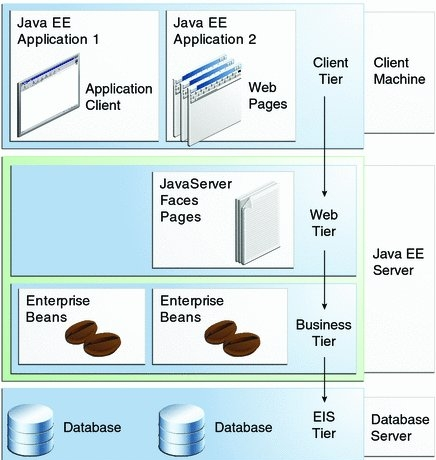
\includegraphics[scale=0.5]{model.jpg} 
\caption{Model Java EE prevzaté z [http://docs.oracle.com/javaee/6/tutorial/doc/].}
\label{model}

\end{center}

\end{figure}
Klient pristupuje k Java EE aplikácií na Java EE serveri z klientskej stanice, prostredníctvom webového prehliadača(\uv{tenký klients} pretože sa nedotazuje priamo na databázový server), alebo klientskej aplikácie, ktorá sa nazýva \uv{hrubý klient}. Tenký klient teda pozostáva z: webové prehliadača, ktorý zobrazuje stránky pozostávajúce z rôzneho značkovacieho jazyka, ktoré sú generované webovými komponentami. Tenký klient sa dotazuje prostredníctvom Hypertext Transfer protokolu(HTTP), čo je internetový protokol pre výmenu hypertextových dokumentov, na webové komponenty na Java EE serveri. Hrubý klient, ktorý môže byť reprezentovaný rozličnými Java SE technológiami pre tvorbu užívateľských rozhraní, sa môže priamo dotazovať podnikových komponent a preskočiť tak komunikáciu s webovými komponentami. \newline \indent Stredná vrstva sa delí na webovú vrstvu, ktorá je prezentovaná technológiami JavaServer Faces a JavaServer Pages. Druhá časť strednej vrstvy takzvaná podniková vrstva býva reprezentovaná technológiu Enterprise JavaBeans, ktoré vytvárajú logiku aplikácie. Webová vrstva je reprezentovaná webovými komponentami, ktoré spracovávajú požiadavky od užívateľa a generujú odpoveď, ktorú posielajú naspäť užívateľovi. Môžu pritom kontaktovať aj podnikové komponenty pre zistenie dodatočných informácií(typicky informácie z databáze). Podniková vrstva je reprezentovaá podnikovými komponentami, ktoré tvoria základ aplikácie. Tieto komponenty môžu prijímať požiadavky od klienta alebo webovej vrstvy a následne generujú odpovede, pričom môžu komunikovať s najnižšou vrstvou(napríklad komunikovať s databázovým serverom). Táto vrstva beží na Java EE serveri. \newline \indent Najnižšia vrstva predstavuje rozličné externé systémy, ktoré aplikácia môže využívať, či už sa jedná o databázový systém, alebo iné. Vrstva býva označovaná skratkou EIS.



\section{JavaServer Pages}\label{jspkap}
JavaServer Pages(JSP) technológia je jazyk, ktorý umožňuje priamo vkladanie Java kódu do HyperText Markup Language(HTLM) kódu. HTML je značkovvací jazyk pre vytváranie webových stránok, ktorý obsahuje HTML značky. Pre vloženia java kódu v HTML stránke sa používajú nasledujúce značky: \emph{<\%} \emph{\%>} medzi, ktoré sa vloží príslušný java kód. Takéto časti v HTML stránke sa nazývaju \uv{skriptlety}. Tieto skriplety sú dynamické, to znamená, že sú vykonávané za behu aplikácie. Behom aplikácie je myslené nasadenie jsp stránky(stránka obsahújca skriplety) na Java EE server, ktorý zabezpečuje jeho vykonávanie prostredníctvom volania jsp kontajneru.

\begin{figure}[htb]

\begin{center}

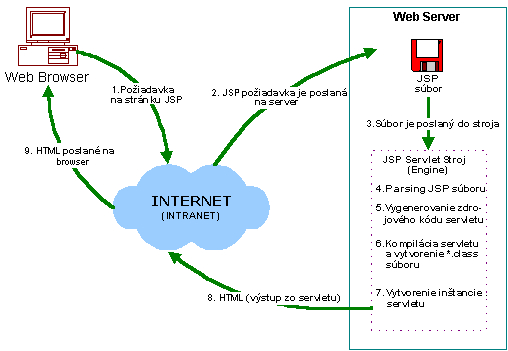
\includegraphics[scale=0.5]{architecture.jpg} 
\caption{JSP architektúra  prevzáte z [http://interval.cz/clanky/javaserver-pages-pro-vsechny/]. }
\label{jsp}

\end{center}

\end{figure}
Na nasledujjúcom obrázku č.\ref{jsp} je zobrazený princíp technológie JSP. Základnou časťou je existenia JSP stránky a jej nasadenie na Java EE serveri. V 1.kroku existuje užívateĺ, ktorý je reprezentovaný webovým prehliadačom, ktorý zažiada o JSP stránku. Java EE server prijme požiadavku od klienta a zistí, že sa jedná o požiadavku o JSP stránku . Ten zavolá JSP servlet kontajner na spracovanie žiadosti, ktorý obsahuje JavaServer Pages prekladač, ktorý obsluhuje spracovanie, kontrolu a generovanie. Následne JSP servlet stroj spracováva JSP stránku a vyhodnocuje skriplety a nahradzuje ich výskytom HTML kódom, ktorý produkuje na výstup. Výstupom zo JSP servlet stroja, ktorý vznikol ako požiadavka o JSP stránku je HTML stránka, ktorá je predaná užívateľovi, ktorý si ju zobrazí. Výhodou tejto technológie je, že pri žiadosť o JSP stránku je, že pri zmene sa nemení celý obsah stránky ale len jej časť, ktorá bola zmenená. Takže takéto JSP stránky sú dynamické a umožňujú zmenu obsahu za behu.



\subsection{JavaServer Faces}\label{jsfkap}
JavaServer Faces(JSF) je framework pre tvorbu užívateľských rozhraní webových aplikácií, ktoré bežia na Java EE serveri\cite{jsfbook}. JSF framework vytvára aplikácie na základe  Model-View-Controller(MVC). MVC predstavuje sotwarovú architektúru, ktorá rozdeľuje aplikáciu na dátový model, užívateľské rozhranie a riadiacu logiku. Princíp je nasledujúci:
\begin{itemize}
\item Model - špecifická reprezentácia dát, s ktorými pracuje aplikácia
\item View - prevádza dáta aplikácie vhodné do podoby prezentácie užívateľa
\item Controller - reaguje na udalosti, typicky od klienta a zabezpečuje zmeny v model alebo view

\end{itemize}
Pri využítí tohto frameworku programátor vkladá predpripravené komponenty(tlačidlá, vyskakovacie okná, rolovacie zoznamy, \ldots) a mapuje ich na príslušné triedy. JSF sa skladá z 2 častí:
\begin{itemize}
\item JSF API - obsahuje komponenty užívateľského rozhrania, umožňuje ich správu, validáciu vstupov, zpracovanie udalostí, navigáciu a iné
\item Knižnica tagov(tag library), ktorá môže byť alternatívne nahradená JSP knižnicou tagov - prostredníctvom týchto špeciálnych tagov vkladáme komponenty užívateľského rozhrania na stránku a upravuje ich chovanie pomocou atribútov alebo mapovaním na triedy. Každá komponenta je definovaná určitou triedou, ktorá určuje jej funkcionalitu. Tagy jednotlivých knižníc sú rozlišované na základe menných priestorov.
\end{itemize}

JSF umožňuje mať výstup v podobe HTML jazyka, alebo iného jazyka v závislosti od definičných tried komponent. Základnou implementáciu prevádza JSF komponenty do HTML kódu.
\subsection{JSF aplikácia}
JSF aplikácia je klasická webová aplikácia, ktorá obsahuje aj svoje špecifiká. Základná štruktúra JSF aplikácie je nasledujúca, pričom nie všetky časti sú povinné:
\begin{itemize}
\item Súbory značkovanie jazyka HTML alebo Extensible Hypertext Markup Language(XHTML)\cite{xhtmlbook}, ktoré obsahuju komponenty užívateľského rozhrania z knižnice tagov, ktoré môžu byť namapované na tzv. \uv{managed bean-y}
\item Managed Beans - java triedy, ktoré sú spravované JSF frameworkom. Najdôležitejšie sú \uv{backing bean}, ktoré zabezpečujú funkcionalitu na HTML/XHTML stránke, udržujú stav komponent, zpracovájú udalosti, validáciu \ldots. Ich konfigurácia sa realizuje v súbore \emph{faces-config.xml}
\item Konfiguračný súbor \emph{faces-config.xml}, v ktorom sa definujú backing beany spolu s ich typom, navigácia, validátory(java triedy, ktorá spracovávajú kontrolujú zadané hodnoty), \ldots
\item Popisovač nasadenia \emph{web.xml}, ktorý umožňuje nastavenie uvítacích stránok, filtre, servlety a \ldots
\end{itemize}
Neoddeliteľnou súčasťou tohto frameworku je Expression Language(EL), je jazyk, ktorý umožňuje dynamicky pristupovať k metódam javovských tried(backing bean). Rovnako dokáže získať a nastaviť hodnotu danej komponenty. Pri preklade sa vygenerejú závislosti na backing beans(java triedy) metódy. Backing bean dokáže za behu spracovávať údaje zadané na webovú stránku, rovnako dokáže obstarať validáciu vstupov,  následne metódy a vlastnosti, ktoré sú volané alebo sú im predávané údaje z vygenerovavnej stránky(HTML alebo XHTML) do backing bean-y alebo opačne. 
V poslednom rade treba uviesť životný cyklus JSF aplikácie.
Celý štandardný cyklus cyklus spracovania požiadavky a následne generovania odpovedi je popísaný na nasledujúcom obrázku.
\begin{figure}[htb]

\begin{center}

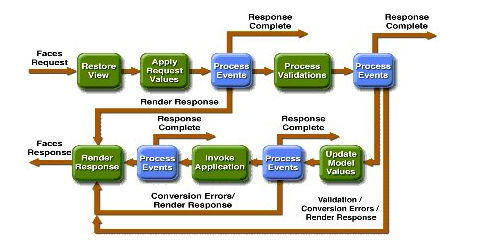
\includegraphics[scale=0.7]{jsflifecycle.jpg} 
\caption{JSF životný cyklus [http://docs.oracle.com/javaee/1.4/tutorial/doc/]. }
\label{lifecycle}

\end{center}

\end{figure}
Na obrázku č.\ref{lifecycle} môžme vidieť životný cyklus JSF aplikácie. Počas fázy Restore View, keď je kliknuté na tlačidlo alebo na link sa vytvorí náhľad stránky, spoja sa všetky spracovania udalostí, validátory a komponenty a uložia sa do inštancie FacesContext. V ďalšej fáze Apply Request Values sú snové hodnoty získané použítím metódy decode. Hodnoty sú potom uložené lokálne do komponenty. Pokiaľ nastane chyba, tak je propagovaná a generovaná do FacesContext-u. Na konci tejto fáze sa vykoná znova dekódovanie. Vo fáze Process Validations spracuje všetky registrované validátory ku komponentám. Pokiaľ nastala chyba, tak je táto informácia uložená do FacesContext-u. Počas ďalšej fázy Update Model Values nastaví do komponent lokálne nové hodnoty. Počas predposlednej fáze Invoke Application sú spracované rozličné žiadosti ako potvrdzonie formulára alebo link na iný stránku. V poslednej fáze Render Response dôjde k renderu stránku s novými hodnotami v kotajnery.

\section{Webová služba}\label{webkap}
Web Service je sotwarový systém navrhnutý na podporu inteoperability medzi rôznymi zariadeniami prostredníctvom počítačovej siete\cite{fitweb}. Komunikácia prebehia prostredníctvom HTTP protokolu vymenieňaním Extensible Markup language(XML) správ. XML je značkovací jazyk, ktorý definuje sadu pravidiel pre kódovanie dokumentu vo formáte porozumiteľnom človeku prostredníctvom ľubovolných značiek. Webové služby poskystujú interoperabilitu medzi rôznymi platformami naprieč počítačou sieťou. Tento aspekt je umožnený tým, že aplikácie komunikujú prostredníctov HTTP protokolu. Komunikácia prostredníctvom webovej služby sa delí na 2 učastníkov. Prvý účastník produkovateľ(producer), ktorý vytvára požiadavok a spotrebiteľ(consumer), ktorý prijíma požiadavok. Komunikácia prebieha medzi týmto dvoma učastníkmi výmenov správ. Webová služba môže byť technicky implementovaný rôznymi možnosťami a prostredníctvom Big Web Service alebo Restful WebService, pričom v princípe ide o java triedy, ktoré obsahujú špeciálne definície triedy a metód a pri nasadení na Java EE server môžu byť vzdialene(po sieti) zavolané ich metódy. 



\subsection{Big webová služba}\label{bigkap}
Big webová služba je druh webovej služby, ktorý pre svoju implementáciu používa API JAX-WS\cite{fitweb} "Big" . Tento typ webovej služby umožňuje vytvárať webové služby orientované na správy alebo techniku vzdialeného volania procedúr(RPC). RPC je technológia, ktorá umožňuje volanie metód, ktoré sa nachádzajú na inom mieste, typicky inom mieste počítačovej siete. Tento typ webovej služby využíva XML správy, spolu so Simple Object Acess Protocol(SOAP) a XML jazykom. SOAP definuje protokol pre výmenu správ založených na jazyku XML prostredníctvom siete prostredníctvom HTTP protokolu. SOAP správy sa skladajú z hlavičky a tela správy, ktoré obsahuje odpoveď webovej služby alebo požiadavok na vyvolanie akcie webovej služby.
\begin{figure}[htb]

\begin{center}

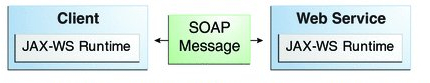
\includegraphics[scale=0.5]{webservice.jpg} 
\caption{\uv{Big} webová služba  prevzaté z [http://docs.oracle.com/javaee/6/tutorial/doc/bnayl.html] }
\label{com}

\end{center}

\end{figure}
Nasledujucí obrázok č. \ref{com} ukazuje spôsob komunikácie medzi klientom, ktorý sa nachádza v ľavej časti obrázku a webovou službou, ktorá sa nachádza vpravej časti obrázku. Komunikácia prebieha prostredníctvom vymienania SOAP správ. Rovnako ako na klientovi tak aj web service obsahuje potrebné API, ktoré spracováva SOAP správy a predáva ich ďalej.

 Tento typ webovej služby obsahuje definíciu vo formáte Web Service Description Language(WSDL). WSDL je definícia vo formáte XML, ktorá popisuje aké akcie webová služba poskytuje a zpôsob ich invokácie, rovnako  aj odpoveď. Správy volania a odpovedí web service sú vymieňané prostredníctvom SOAP správ prostredníctvom HTTP protokolu. JAX-WS API je pomerne komplikované, preto celá komplexnosť je vývojarovi zakrytá a je jediné, čo definuje vývojár sú metódy, ktoré je možné vzdialene volať. Rovnako vývojár nespracováva SOAP správy, ale celá táto problematika je riešená prostredníctvom prostredníctvom API. API umožňuje prístup k ne-Javovským web service, čo prináša veľkú flexibilitu. Čo sa týka vývoja web service, tak sa jedná o jednoduchú Java triedu, ktorá používa anotáciu javax.jws.WebService, konkrétne anotáciu @WebService, ktorá označuje, že sa jedná o konvocý bod webovej služby. Táto trieda následne definuje metódy, ktoré môžu byť vzdialené volané. Aby moha byť metóda metódou webovej služby musí byť anotovaná prostredníctvom anotácie  javax.jws.WebMethod @WebMethod.

\subsection{RESTful webová služba}\ref{restkap}
RESTful webová služba je druh webovej služby, ktorý pre svoju implementáciu používa API JAX-RS\cite{fitweb}. Tento druh webovej služby nevyžaduje striktné používanie XML formátu a doručovanie správ vo formáte SOAP. K tomuto typu webovej služby je pristupované na základe Uniform Resource Identifier(URI), ktorý predstavuje textový reťazec, ktorý slúži k špecifikácií zdroja. K tomuto je používaná anotácia @Path(), ktorej hodnota zabezpečí namapovanie a teda pomocou nej môžme pristupovať k RESTful webovej službe. Keďže táto služba nemá presne stanovený formát správ môžeme zvoliť z formátov ako HTML,JSON, PDF, \ldots. Tento typ služby je bezstavový, takže každý prístup musí obsahovať všetky potrebné informáce, pričom je možné ich označiť ako cachovatelné(uchávajúcée sa vo vyrovnávanej pamäti) kvôli zvýšeniu výkonosti. Nevýhodou je, že pri vytváraní klienta a služby musí byť použité rovnaké rozhranie z dôvodu explicitnej nepodporovateľnosti jednoznačného formátu správy pre komunikáciu.


\section{Princíp webových komponent}
Java EE webové komponenty sú softwarové komponenty, ktoré spracovávajú prichádzajúci HTTP požiadok a poskytujú naň odpoveď. Všetky Java EE webové komponenty sú postavané na servletoch. Servlety sú javovské triedy , ktoré dynamicky spracovávajú požiadavky a tvoria odpovede. Súčasťou servletov alebo webových stránok  sú technológie JavaServer Faces technológiu(JSF)\ref{jsfkap} and JavaServer pages(JSP)\ref{jspkap}. Technológie JavaServer Faces a JavaServer Pages podporujú spracovanie užívateľských vstupov a ich predanie a spracovanie podnikovou vrstvou.



\begin{figure}[htb]

\begin{center}

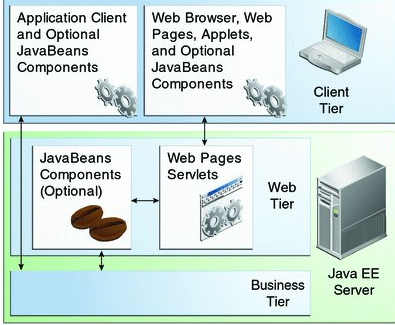
\includegraphics[scale=0.5]{webtechnology.jpg} 
\caption{Webové komponenty prevzáte z [http://docs.oracle.com/javaee/6/tutorial/doc/bnaay.html]. }
\label{web}

\end{center}

\end{figure}
Na nasledujúcom obrázku č.\ref{web} je ukázaný princíp fungovania webových komponent. V hornej ľavej časti obrázku sa nachádza klientská vrstva, ktorá obsahuje buď len webový prehliadač po prípade Applety. Applet je aplikácia, ktorú spúšťa užívateľ prostredníctvom webového prehliadača a je vykonávaná virtuálnym strojom. V hornej pravej časti môže byť klient reprezentoný aplikačným klientom, ktorý obsahuje obsahuje úplnú prezentačnú logiku aplikácie a teda v tom prípade, odpadá potreba spracovania vstupov webovými komponentami. Takýto klient komunikuje už len priamo s Java EE serverom, konkrétne podnikovou vrstvou, ktorá implementuje zvyšnú logiku aplikácie. V prípade, že máme k dispozícií tenkého klienta, klient komunikuje prostredníctvom webové prehliadača s HTML alebo XHTML stránkami, ktoré sú vytvorené technológiou JavaServer Faces\ref{jspkap} alebo JavaServer Pages\ref{jspkap}, ktoré spracovávajú požiadavky od klienta(vstupy) a následne komunikuje s podnikovým stupňom, ktorý obsahuje logiku aplikácie, ktorá následne môže komunikovať s databázovým serverom. Odpoveď je v prípade tenkého klienta následne \uv{predaná} stránkám vytvoreným prostredníctvom JavaServer Faces alebo JavaServer Pages technológiou a následne zobrazená užívatelovi v podobe výstupu webovej stránky. V prípade hrubého klienta sa výstup zobrazí v aplikačnom klientovi.


\section{Java Persistence API}\label{jpakap}
Java Persistence API(JPA) je framerok jazyku Java, ktorá poskytuje prístup a spravovanie dát v databázy pomocou prístupu \emph{objektovo relačné mapovanie}\cite{jpabook}. JPA obsahuje API, ktoré je nezávislé nad použitou databázou technológiou, je možné vytvárať dotazy nad MySQL, SQL databázou, \ldots. Tento prístup  umožňuje mapovanie dát medzi  z databázových tabuliek na objekty javy(entity). Entita je základnou jednoutou JPA, s ktorým pracujeme pri manipulácia s dátami. Entitna je je odľahčený perzistentný doménový objekt, ktorý typicky reprezentuje tabuľku v relačnej databázy a každá jej inštancia je riadkom v  tabuľke. Základný artefaktom v programovaní je pre entity entitná trieda, ktorá obsahuje vlastnosti, ktoré priamo odpovedajú schéme vytvorenej databáze. Každá entitná trieda musí spĺňať určité kritéria:
\begin{itemize}
\item Entitná trieda musí byť anotovaná javax.persistence.Entity anotáciou. Anotácia je reťazec obsahujúci znak \emph{@} nasledovaný ľubovolným nenulovým počtom znakov, pričom môže v zátvorkách obsahovať ďalšie parametre. Anotácia pridáva ďalšie informácie o označenej(anotovanej položke). Anotovať môže rovnako metódy, triedy ale aj vlastnosti tried.
\item Entitná trieda musí mať parametrický konštruktor, aby bolo možné vytvárať nové entity
\item Každá vlastnosť entitnej triedy musí spĺňať princíp Plain Old Java Objec(POJO), čo znamená, že pre každú vlastnosť existuje metóda v tvare getNázovVlastnosti, ktorá získa hodnotu vlastnosti a metóda v tvare setNázovVlasnosti, ktorá nastaví danú hodnotu vlastnosti. Jednotlivé vlastnosti môžu byť dodatočne anotované napr. kvôli kontrole na hodnotu konkrétneho typu alebo vlastnosti(nenulovosť, špeciálny formát, \ldots).
\item Každá entitná trieda musí mať mať unikátny identifikátor. Týmto identifikátorom chápeme primárny kľúč, čo je vlastnosť, ktorá dokáže v databáze jednoznačne identifikovať záznam. Primárny kľúč býva anotovaný prostredníctvom anotácie javax.persistence.Id
\end{itemize}

Rovnako treba spomenúť, že každá entitná trieda môžu byť vo vzťahu s inými entitami. V prípade, že vlastnosť entity je súčasťou vzťahu s inou entitou použijeme niektorú z nasledujúcich anotácii podľa násobnosti vzťahu: \emph{@One-to-one, @One-to-many, @Many-to-one, @Many-to-Many}. Rovnako uvedenie vlastnost/vlastnosti druhej entity, ktoré sa podieľajú na vzťahu. To urobíme tak, že našu vlastnosť ešte anotujeme anotáciou javax.persistence.JoinColumn, v ktorej parametroch uvedieme názvy vlastnosti druhej entity, ktoré sú súčaštou vzťahu.
JPA ponúka aj iné, pokročilé možnosti mapovania, pre naše potreby nám budú stačiť nasledujúce informácie.
\newline \indent Aby sme mohli s entitami pracovať potrebujeme si vytvoriť inštanciu triedy javax.persistence.EntityManager. EntityManager je trieda, ktorá dokáže vytvárať a odstraňovať entity, umožňuje ich vyhľadávať, rovnako aj vytvárať dotazy nad databázou. Dotazy, ktoré môžme vytvoriť pomocou JPA sa podobajú klasickému jazyky Structured Query Language(SQL), ktorý dokázaže vytvárať dotazy nad databázou, avšak dotazovací jazyk jazyk JPA má niekoľko rozdielov. Tento jazyk sa nazýva Java Persistence Query Language(JPQL), čo je ako bolo spomenuté jazyk podobný SQL, pričom tento jazyk je reťazcovo založený a je nezávislý na zvolenej databázovej techológií a má objektové vlastnosti, čo znamená, že pri tvorbe dotazovou používame názvy vlastností entitných tried a názvy entitný tried. Problém JPQL je typová nebezpečnosť, čo vyžaduje pretypovanie výsledkov dotazu z entity manager-a. To môže spôsobiť chyby, ktoré nemusia byť odchytené počas kompilácie. JPA definuje ešte Criteria API, ktoré je využívané k vytváraniu dotazovou nad entitami a vzťahou, ktoré sú typovo bezpečné. Výhodou tohto API, pre použitie na dotazovanie, je rovnako možnosť vytvárať dynamické dotazy, ktoré majú lepšiu výkonnosť ako JPQL. Aby EntityManager bol schopný pracovať s určitými entitnými triedami je nutné vytvoriť \emph{perzistentnú jednotku(persistence unit)}, čo je XML predpis, do ktorého uvedieme entitné triedy, odkaz na databázu po prípade ďalšie vlastnosti a ten vložíme do súboru persistence.xml. Tento súbor predstavuje konfiguráciu, ktorá obsahuje okrem názvu entitných tried, tak aj rôzne iné vlastnosti, napr. je možné automaticke vytvoriť schému databáze z entitných tried. V tomto súbore sa rovnako nachádza doležitá položka a to je datasource, ktorý definuje odkaz na databázu, s ktorou pracujeme. Na záver kapitoly zhrniem princíp práce s JPA:
\begin{itemize}
\item Vytvorenie entitných tried spolu s vlastnosťami, správne naanotovanie tried, pričom návrh entitných tried odpovedá návrhu schémy databáze, ktorý požadujeme
\item Registrácia entitných tried v súbore persistence.xml, v ktorom nastaví aj odkaz na nami používanú databázu
\item Vytvorenie inštancie triedy EntityManager, pričom môžme explicitne uviesť názov perzistentnej jednotky, s ktorou pracujeme(perzistentných jednotiek môže byť viac)
\item Pracujeme s databázou spôsobom vytváraním, mazaním, editovaním hodnôt entitných tried, ktoré zapisujeme do databáze EntityManager-om, alebo vytvárame dotazy, ktoré realizuje EntityManager-om a výsledky podľa potreby spracovávame.
\end{itemize}


\section{Enterprise JavaBeans}\label{ejbkap}
EnterpriseJavaBeans(EJB) je technológia, ktorá umožňuje vytvárať komponenty, ktoré bežia v strednej, konkrétne podnikovej vrstve aplikačného modelu Java EE\cite{ejbbook}\ref{kapapp}. Takéto komponenty sú modulárne, keďze je možné ich vytvoriť a spravovať viac inštancií a môžme do nich umiestniť logiku našej aplikácie. Takéto komponenty komunikujú s klientom alebo webovými komponentami a na druhej strane môžu komunikovať s EIS vrstvou a vykonávajú/predávajú získané informácie. Na EJB sa môžme pozerať aj ako na API platformy Java EE, prostredníctvom, ktorého môžme vytvárať triedy, ktoré sú špeciálne anotované a obsahujú podnikovú logiku a sú nasadené na Java EE server. Základnou podmienkou nasadenia na Java EE server je prítomnosť EJB kontajneru, do ktorého sa inštalujú vytvorené triedy. Triedy vytvorené týmto API nazýva \emph{Enterprise Bean-y(EB)}.

EB sa delia na 2 kategórie:
\begin{itemize}
\item Message-driven bean - Pôsobí v roli poslucháča  určitého typu správ, na ktorých príjem reaguje vykonaním určitých akcií\cite{fitweb}
\item Session bean - Vykoná úlohy pre klienta. Môže implementovať webové služby\cite{fitweb}

\end{itemize}


\subsection{Session Bean}\label{sessionkap}
Session bean(SB) je typ EB, ktorá zapúzdruje podnikovú logiku, ktorá môže byť vyvolaná lokálne alebo vzdialene. Prístup k session bean je realizovaný prostredníctvom volania metód SB. SB následne vykoná kód metódy, po prípade vráti nejaký výsledok. \newline \indent SB môže byť 3 typov:
\begin{itemize}
\item Stateful Session Bean - beany udržuje hodnoty premených, každá beana reprezentuje unikátny stav klienta/bean sedenia. Pokiaľ sa sedenie odstrániť stav zmizne.
\item Stateless Session Bean - Neudržuje stav komunikácie s klientom. Počas invokácie metódy takejto beany môže inštancia obsahovať premenné, ktoré môžu obsahovať špecifický stav vzhľadom na klienta, alebo len počas invokácie metódy. Stav po ukočení mizne, rovnako tento typ SB je možné použiť k implementácií webovej služby.
\item Singleton Session Bean - Teto typ beany je inštanciovaný len raz a pretrváva počas celého životného cyklu aplikácie. Využíva sa pri zdieľaní a súčasnom prístupe viacerých užívateľov.
\end{itemize}

\subsection{Message-driven Bean}\label{messagekap}
Message-driven bean(MB) je typ EB, ktorá umožňuje Java EE aplikáciám asynchronné spracovanie správ. Tento beany prijíma Java Messaging Services(JMS) správy z JMS fronty, ktoré následne analyzuje a vykonáva akcie\cite{jmsbook}. JMS je technológia, ktorá umožňuje komunikovať komponentám prostredníctvom správ. JMS fronty sú obyčajné fronty, do ktorých sa na jednom konci pri zavolaní MB vloží špecifická JMS správa a na druhej strane je MB postupne tieto správy odoberané a teda spracované len raz. JMS správa obsahuje rôzne informácie(špecifické hodnoty, \ldots). Správy zaradené v JMS fronte môžu byť poslané rôznymi Java EE komponentami, alebo aj iným systémom, ktorý nepoužíva Java technológiu. Zásadny rozdiel je oproti session bean v zásade v tom, že sa k takému  typu beanu nepristupuje prostredníctvom rozhrania a invokácie metód.Prístup k takému typu EB sa deje prostredníctvom vytvorenia spojenia s JMS frontou a vložení správou do fronty. Správy sú následne spracované na strane MB metódou \emph{onMessage}, ktorá vyberá z JMS fronty správu po správe. Výhodou MB je ekvivaletnosť MB, to znamená že správy môže EJB kontainer ľubovoľnej inštancii. MB má môžu byť vyvolané asychrónne, ktoré nevyťažujú tak prostriedky servera, žijú relatívne krátko a sú bezstavové. 

\section{Twitter Bootstrap}\label{bootkap}
Twitter Bootstrapje je dostupný súbor nástrojov pre vytváranie webových stránok a webových aplikácií\cite{boot}. Ponúka podporu najrôznejších webových technológií HTML, CSS, JavaScript a mnoho prvkov, ktoré je možné ľahko integrovať do svojej stránky. Boostrap implementuje interaktívne prvky ako sú tlačidlá, boxy, menu a ďalšie grafické elementy. Pre použitie Boostrap-u je potrebné vložiť do HTML kódu odkaz  na  kaskádové štýly a javascriptový súbor.

Výhodou týhto nástrojov je jednoduché používanie a možnosť použitia aj na mobilných telefónoch. Podrobné vysvetlenie jednotlivých komponent nájdete na nasledujúcej adrese http://getbootstrap.com/, rovnako aj s príkladmi použitia. 

Boostrap obsahuje rozšírenie Font Awesome, čo je CSS framework, ktorý obsahuje rôzne grafické ikony, ktoré je možné intregovať do HTML kódu\cite{fontweb}.


\section{Rich Faces}\label{richkap}
Rich faces je open-source framework s podporou Asynchrouns Javavascript and\\ XML(AJAX)\cite{ajaxbook}, ktorý predstavuje rozšírenie JSF frameworku \ref{jsfkap}. Rich Faces obsahuje API, ktoré obsahuje grafické komponenty s podporou Ajax-u. RichFaces podporuje množstvo preddefinovaných vzhľadov. Rovnako umožňuje definovať, ktoré JSF komponenty budú invokované na základe Ajax požiadavky, vrátane spôsobu invokácie a odpovede. Rovnako podporuje validáciu na strane klientského prehliadača.


\section{MySQL}\label{mysqlkap}
MySQL je databázová technológia, ktorá je vhodná pre malé a stredne veľke aplikácie, rovnako poskytuje dobrý výkon pri vykonávaní transakcíí. Umožňuje vytvárať procedúry, databázové triggere a jej inštalácia je pomerne jednoduchá a nezaberá veľa diskové priestoru. Rovnako je MySQL multiplaformová, keďže je možné ju nasadiť na systémy s operačným systémov Windows, Linux, Mac Os. Medzi nevýhody tejto technológie patrí neefektívna práca s databázovými transakciami, neefektívne ukladanie veľkého množstva dát. MySQL je open source a je vyvíjaná spoločnosťou Sun Microsystems.

\section{Seam}\label{seamkap}
Seam je aplikačný framework pre Java EE, ktorý definuje uniformný komponentný model pre podnikovú logiku aplikácie\cite{seambook}. Seam rieši integráciu EJB\ref{ejbkap} a JSF\ref{jsfkap} spolu. Medzi ďalšie výhodné vlastnosti tohto frameworku patrí integrácia Asynchronous JavaScript and XML(Ajax)\cite{ajaxbook}, rovnako aj vstavaná podpora javascriptu a efektívne spracovanie webových dotazov. \newline \indent Modul Seam security, ktorý obsahuje množstvo mechanizmov na zabezpečenie enterprise aplikácie. Základom každej bezpečnosti je autentifikácia, čo je process vytvorenia alebo potvrdenia identity užívateľa. Užívateľ potvrdzuje svoju identitu prostredníctvom užívateľského meno a hesla. Seam security poskytuje API prostredníctvom, ktorého je možné sa autentizovať z rozličných zdrojov(databáze, \ldots). Ďalšou vlastnosťou je Identity Management, ktoré je množina API na správu užívateľov, skupín a užívateľských rol. Identity Managent je poskytovaný Seam komponentou PicketLink IDM, ktorá spravuje uloženie užívateľov v rozličných bezpečnostných úložiskách. \newline \indent Základom autentifikácie je Identity Bean, čo je java trieda, ktorá reprezentuje identitu užívateľa a pri úspešnej autifikácií je identita je vložená do životného cyklu aktuálneho sedenia. V rámci autentifikácie sú definované metódy \emph{Login(prihlásenie)} a \emph{Logout(odhlásenie)}. Základom každej triedy, ktorá realizuje autentifikáciu je metóda(authenticate), v ktorej prebieha autentifikácia uźívateľa.
Počas autentifikácia sa overí pravosť užívateľa a prostredníctvom metódy \emph{setStatus} sa nastaví úspech(SUCESS) alebo neúspech(FAILURE) pri overení zadaných údajov. Po autentifikácií dôjde k vloženiu identity užívateľa do životného cyklu aplikácie, ktorú je možné získať z triedy triedy prostredníctvom anotácie @Inject triedy Identity.
\newline \indent Ďalší modul, ktorý nás zaujíma je Seam Faces, ktorý obsahuje API na zabezpečenie prístupu k HTML a XHTML stránkám. Túto fukčnosť nazývame \emph{Faces View Configuration}, ktorá nám umožňuje spojenie so Seam Security modulom na obmedzenie/povolenie prístupu pre danú užívateľskú rolu, preprepisovanie URL\ldots. Seam framework patrí pod divíziu JBoss, takže je pomerne jednoduché ho intergrovať pod aplikačný server JBoss-u. 


\section{Testovanie}\label{testkap}
V poslednom rade uvedieme technológie, ktoré budeme používať pre testovanie. Základom testovania je nástroj JUnit a nástroj Arqullian.
V prvom rade sa budem venovať nástroju JUnit. JUnit je unit testovací nástroj pre programovací jazyk Java. JUnit sa používa pre typ testovania, ktorý sa nazýva \uv{test-driven development}\cite{testdevbook} a je jedným z kolekcie unit testovacích nástrojov. JUnit býva súčaštou balíku org.junit\cite{junitbook}. Testovacie metódy sú anotované prostredníctvom @Test anotácie. JUnit rovnako umožňuje vykonať kód pred spustením testu, to docielime anotovaním metód @Before anotáciou alebo po sputení testu, to docielime anotáciou @After. V testovacej metóde potom vykonáme nejaké kód a očakávaný výstup porovnáme s nami očakávaným výsledok prostredníctvom metódy \emph{Assert}. JUnit testy sú písané pre otestovanie konkrétnej funkčnosti kódu. Cieľom testovania prostredníctvom JUnit sú malé kúsky kódu, ako metódy alebo triedy. 
\newline \indent Nakoniec spomeniem nástroj Arquallian. Arquallian je testovací nástroj, ktorý vykonáva testy vo vnútri vzdialeného alebo vstavaného kontajneru alebo nasadí archív(obsahujúci java triedy spolu s testovacími trieda) na Java EE kontajner. Arquallian integruje aj ďalšie testovacie nástroja, napr. JUnit 4, TestNG 5, \ldots. Treba zdôrazniť, že narozdiel od JUnit testov umožňuje testovanie v java EE kontajnery(GlassFish, JBoss)\cite{arqbook}. Tento framework má zásadnú výhodu v prenositeľnosti testov na rôzne podporované Java EE kotajnery. Nástroj pri spustení automaticky zabalí do archívu všetky potrebné prostriedky pre platformu. 
\newline \indent Použitie Arqullian sa deje použitím anotácie @RunWith Arquillian v našej javovskej testovej triede, ktoré zabezpečí spustenie testov. Následne tento nástroj spustí kontajner a nasadí testovací archív, ktorý je daný anotáciou @Deployment. Archív obsahuje testy so špecickými triedami a knižnicami. Testy sa následne vykonajú vo vnútri kotajneru. Čo znamená, že môžu otestovať podnikové a webové komponenty za behu. Písanie testo s nástrojou Arqullian začína tvorbou javovskej triedy, ktorá vyzerá ako štandardná testovacia trieda vytvorená nástrojom JUnit, pričom obsahuje vyššie spomenuté špecifické anotácie, ktoré umožňujú pri spustení testu vytvorenie archívu, nasadenie na Java EE kontajner a následne spustenie testov. V poslednom rade je potrebné nakonfigurovať v XML súbore arquillian.xml pre použitie Java EE kontajnera. Arquallian.xml je XML súbor, ktorý obsahuju použitie Java EE kontajneru a ďalšie špecifické vlasnosti.


\section{WildFly Aplikačný server}\label{jbossc}
Aplikačný server(AS) je sotware, ktorý poskytuje vrstvu medzi operačným systémom a Java EE aplikáciami. AS poskytuje funkcionalitu aplikáciám(prístup k súborovému systému, \ldots), konkrétne enterprise aplikáciám. Vytvára vrstvu, ktorá zjednodušuje vývoj enterprise aplikácie. Pomerne veľká skupina AS je vyvíjaná v jazyku Java. Dôvodom pre tento jazyk je existencia štandardu Java EE.

WildFly je open-source aplikačný server verzie 8, ktorý vznikol premenovaním aplikačného serveru JBoss, čo je vlastne skratka pre JavaBeans Open Source Applicatom Server. Pre naše potreby budeme používať WildFly v verzii 7, preto bude používaný názov JBoss. JBoss je aplikačný server, ktorý je založený na platforme Java a Java Enterprise Edition.\cite{jbossbook}. Tento typ AS je open-source, preto je možné jeho stiahnutie spolu so zdrojovými kódmi. Používanie aplikačného servera JBoss je veľmi jednoduché jeho spustenie môžte vykonať ručne prostredníctvom konzole a nájdeným inštalačného adresára, ktorý obsahuje skript run.sh, ktorý spustí JBoss. Po spustení serveru je možné k nemu implicitne pristupovať na localhost na porte 8080. Základným stavebným kameňom JBoss AS je JBoss Microcontainer. JBoss Microcontaijner je refaktorizácia JBoss JMX Microkernel aby podporoval POJO nasadzovanie a samostatné použitie mimo aplikačného servera. Microcontainer registruje všetky použité služby. Služby, ktoré majú by prístupné sa registrujú v podobe managed beans. Microcontainer spravuje a riadi beh týchto služieb. JBoss je licensovaný pod GNU Lesser General Public License(GNU PL).


\chapter{OptaPlanner}\label{optaplannerC}
OptaPlanner je open source framework a prokračovanie frameworku JBoss Drools, ktorý vykonáva a optimalizuje rôzne plánovacie problémy, ktoré sú reprezentované XML súborom, s rozličným stupňom náročnosti. Optaplanner využíva pri riešení problému, ktoré nemusí vždy nájsť, optimalizačné algoritmy a metaheuristické metódy s využitím skóre. Skóre je hodnota, ktorá reprezentuje bodové hodnotenie optimálnosti dosiahnutého riešenia. Výsledným riešením je to riešenie, ktoré má najvyššie skóre. Tento framework neurčuje striktne akými algoritmami a metódami sa má daný problém vyriešiť, ale konfiguráciu ponecháva na strane užívateľa. OptaPlanner je určený pre jazyk Java, preto riešenie je vykonávané triedami v tomto jazyky. Tieto triedu sú špecifické pre daný problém, a musia byť schopné získať potrebné informácie z defičného súboru problému, ktorý reprezentuje zadanie problému, musia byť schopné vykonávať postupné kroky vedúce k riešeniu problému(napr. v prípade problému N Dám presúvať dámy, tak aby sa vždy nachádzali vo validných pozíciách) a prostriedky, ktoré ohodnotnia krok a prekalkulujú celkové skóre. \newline \indent Samozrejme postup riešenia problému, kalkulácií skóre sa opakuje pre rôzne scenáre(napr. v prípade N Dám pre rôzne alternatívne kombinácie pohybov) a vráti sa riešenie s najlepším skóre v podobe súboru vo formáte XML(napr. v prípade riešenia problému N Dám poskytne najlepšie možné riešenie rozmiestnenia). OptaPlanner sa snaží vždy nájsť optimálne riešenie vzhľadom k optimalizačným algoritmom a metaheurestickým metódom a dostupnému času, ale niekedy nie je schopný poskytnúť na predchádzajúce podmienky optimálne riešenie(riešenie je ukončené predčasne z dôvodu vyčerpania dostupného času). Výhodou tohto frameworku je možnosť aplikovania na NP-úplne problémy(ktoré sú riešené v dostupnom časom). 

\section{Plánovací problém}\label{planprob}
Plánovacím problémom môžme obecne rozumieť akýkoľvek problém, ktorý vyžaduje od nás zdroje a predikciu na priradenie zdrojov, nájdenie riešenia takého, aby výsledok bol v konečnom dôsledku najlepší, cenovo aj časovo najprijatelnejší.

V bežnom živote, rovnako ako ja v podnikových sférách sa stretávame s rôznymi plánovacími problémami. Môže ísť o problémy ako správne naplánovať cestu vozidiel(aút, lodí,\ldots), aby sme ju spravili za čo najkratší čas, rovnako môžme požadovať aby cesta bola, čo finančne najefektívnejšia. Rovnako môžme plánovať rozvrh práce zamestatnancov vo firme, aby zbytočne nespomalovali chod ostatních zamestatnci, ktorí sú na ich práci závislí a nemuseli zbytočne čakať. Plánovať môžme spúšťanie testovania aplikácií v rámci vývojarskej firmy, aby niektoré úlohy boli otestované skôr ako iné, no musí byť čo najefektívnejšie vývažené a zbytočne nemrhali časovým kvantom. Pokiaľ je problém dostatočne komplexný potom je veľmi vhodné použiť Optaplanner. 

\begin{figure}[htb]

\begin{center}

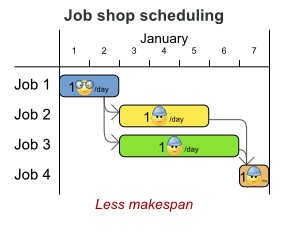
\includegraphics[scale=0.8]{fig/useCaseOverview.jpg} 
\caption{Problém rozvrhnutia práce, prevzaté z [http://www.optaplanner.org/]. }
\label{obrazokUseCase}

\end{center}

\end{figure}
Obrázok č. \ref{obrazokUseCase} zobrazuje typické použitie OptaPlanner-u. Môžme vidieť v nasledujúcom obrázku vystupujú 4 osoby(označené obdĺžnikom modrej, žltej, zelenej a oranžovej farby), ktoré vykonávajú nejakú činnosť. Ich činnosť je špecifická a silne závisí od práce predchádzajúcich. V prípade náročnosť zadania takého problému je pomerne jednoduché naplánovať správne poradie činností. Problém nastáva, ak by v danom obrázku bolo niekoľko násobne viac ôsob. V tomto prípade štandardným prístupom by mohlo dôsť k neefektívnemu rozdelnie práce a k zbytočnému mrhaniu času. Preto je vhodné použiť OptaPlanner, ktorý sa snaží ich činnosti maximálne optimalizovať a jednotlivé činnosti zvoliť v následnosti tak, aby výsledná práca bola spravená za najkratší možný čas vzhľadom na činnosť, ktorá sa optimalizuje.

Definícia problému v prirodzenom jazyku by mohla v oblasti informačných technológií spôsobiť nejednoznačnosť v jej interpretácií, preto je používaný súbor vo formáte XML, v ktorom definujeme počiatočné zadanie  plánovacieho problému. Formát XML súboru závisí od zadania problému. V prípade, že si zobere problém N Dám, tak zadanie súboru obsahuje presnú pozíciu dám na šachovnici. Keď si zobereme problém obchodného cestujúceho, tak definičný XML súbor obsahuje zoznam miest a jednotlivé vzdialenosti od seba. Obsah definičného súboru nemá jednoznačný formát, ale vždy závisí od plánovacieho problému.


\section{Výsledky plánovacieho problému}
OptaPlanner podporuje niekoľko optimalizačných algoritmov ako efektívne nájsť tieto veľké množstvá riešení. V závislosti na prípade použitia, niektoré optimalizačné algoritmy dosahujú lepšie výsledky ako ostatné, ale to je nemožné povedať dopredu. Pri plánovaní, je ľahké prepnúť algoritmus optimalizácie, zmenou konfigurácie. Rovnako je možné rozpracovať viacero riešení problému prostredníctvom rôznych plánovacích algoritmov a metaheurestických metód, pričom je poskytnuté riešenie s najlepším skóre reprezentované XML súborom.



\section{Princíp}
Princíp riešenia problému je založené na konfigurácií OptaPlanner tvorbou javovských tried na získanie potrebných dát z definičného súboru, prostriedkov na kalkuláciu skóre a aplikáciu odkiaľ sa spúšťa výpočet. Riešenie problémom sa začína tvorou XML definičného problému špecifického pre daný problém. Následne sa vytvoria triedy pre získanie dát z XML súboru, triedy pre vykonávanie krokov plánovania(napr. v prípade N dám presúvanie dám na validné pozicie) a prostriedky pre kalkuláciu skóre a nastavenie konfiguračného súboru pre daný problém, ktorý bude bližšie popísaný v nasledujúcej kapitole\ref{confopt}. Aby bolo jasné aké akcie sú povolené pre daný problém sú definované v triedach pre riešenie obmedzenia:
\cite{optabook}
\begin{itemize}
\item Negatívne "hard" obmedzenie, ktoré nesmú byť porušené\label{hardobm}
\item Negatívne "soft" obmedzenie, ktoré by nemali byť porušené pokiaľ sa dá tomu vyhnúť.
\item Pozitívne "soft" obmedzenia, ktoré by mali splnené pokiaľ je to možné(môžu viesť k lepšiemu skóre)
\end{itemize}

 Prostriedky pre kalkulácie skôre môžu byť 3 typov:
\begin{itemize}\label{skorkal}
\item Jednoduchá kalkulácie skóre 1 metódou
\item Inkrementálna kalkulácie skóre prostredníctvom viacerých metód
\item Drools kalkulácia skore - táto konfigurácia definuje pravidlá pre kalkulovanie skóre\label{drollskal}
\end{itemize}
Drools kalkulácia skóre využíva vlastnú DRL syntax a je daná súborom, ktorý obsahuje pravidlá. Každé pravidlo je dané svojim názvom a podmienkou, v ktorej sa overuje priebežné riešenie problému(napr. v prípade N Dám priebežné rozloženie dám), ktorá v prípade splnenia upravuje skóre. Treba zdôrazniť, že v konfiguračnom súbore užívateľ nastavuje optimalizačné algoritmy a metaheuristické metódy, ktorý sa snažia v spolupráci s triedami na riešenie vyberať vždy najlepšie kroky pri riešení.

 Spustenie riešenia je dané zavolaním hlavnej metódy odkiaľ sa spúšťa riešenie problému. 
a spustí vykonávanie(plánovanie). Postup je nasledovný:
\begin{enumerate}
\item Overenie prostriedkov(definičného súboru, konfiguračného súboru(obsahuje spôsob kalkulácie, definičného triedy, použitie plánovacích algoritmy a metaheurestických metód) a prostriedkov na kalkuláciu skóre)
\item Načítanie obsahu XML súboru 
\item Vykonanie kroku podľa použitia plánovacích algoritmov
\item Optimalizácia kroku v prípade použitia metaheuristických metód
\item Ohodnotenie kroku(v závislosti od použitia prostriedkov na kalkuláciu skóre\ref{skorkal})
\item Vykonanie alternatívneho kroku vzhľadom(napr. v prípade N Dám presunutie dámy na ľavú stranu šachovnice, miesto pravej)
\item Optimalizácia alternatívneho kroku v prípade použitia metaheuristických metód
\item Ohodnotenie kroku(v závislosti od použitia prostriedkov na kalkuláciu skóre\ref{skorkal})
\item Opakovanie krokov 3., 4., 5., 6. až dokým nie je dosiahnuté riešenie alebo plánovanie nie je predčasne ukončené
\item Nájdenie riešenia alebo predčasné ukončenie plánovanie vzhľadom na vysoké poskytnuté skóre(je možné použiť v prípade, že riešenie problému nebolo nájdené v dostupnom čase)

\end{enumerate}

\newpage
\section{Konfiguráciu OptaPlanneru}\label{confopt}
Konfigurácia OptaPlanner sa realizuje prostredníctvom XML súboru, ktorá má 3 povinné časti a 4. voliteĺnú. Pre lepšiu prehľadnosť je uvedená ukážka konfiguračného súboru. 
 \lstset{
    language=xml,
    tabsize=3,
    %frame=lines,
    caption=Vyváženie cloudu,
    label=code:sample,
    frame=shadowbox,
    rulesepcolor=\color{gray},
    xleftmargin=20pt,
    framexleftmargin=15pt,
    keywordstyle=\color{blue}\bf,
    commentstyle=\color{OliveGreen},
    stringstyle=\color{red},
    numbers=left,
    numberstyle=\tiny,
    numbersep=5pt,
    breaklines=true,
    showstringspaces=false,
    basicstyle=\footnotesize,
    emph={food,name,price},emphstyle={\color{magenta}}}
    \lstinputlisting{cloudBalancingSolverConfig.xml}

\newpage
Nastavenie konfiguračného súboru(solver) pre riešenie problému vyváženie cloudu pozostáva z 3 častí: 
\begin{itemize}
\item Nastavania definičných tried plánovacie problému, nastavania tried zabezpečujúce plánovanie, nastavenie definícií skóre a nastavenie použitia plánovacích algoritmov, po prípade nastavenia metaheurestických metód
\item Súbor je rozdelený na 3 časti:
\begin{itemize}
\item Domain model configuration(začínajúc riadkom č.4), v ktorom sú uvedené triedy definujúce problém a riešenie
\item Score Configuration(začínajúc riadkom č.7) definujúce spôsob kalkulácie skóre vrátane triedy
\item Optimalization algorithms configuration(začínajúc riadkom č.13) sú uvedené optimalizačné algoritmy, vrátane spôsobu ukončenia plánovia
\end{itemize}
\item Na riadku č.3 uvedená medzi značkami \emph{enviromentMode} hodnota \uv{FAST\_ASSERT}, ktorá umožňuje OptaPlanner detekovať chyby v implementácií
\item Na riadku č.5 je uvedená medzi značkami \emph{solutionClass} hodnota \\\uv{org.optaplanner.examples.cloudbalancing.domain.CloudBalance}, ktorá odkazuje na definičnú triedu modelu problému vyváženie cloudu
\item Na riadku č.6 je uvedená medzi značkami \emph{planningEntityClass} hodnota \\\uv{org.optaplanner.examples.cloudbalancing.domain.CloudProcess}, ktorá odkazuje na triedu, ktorá realizuje riešenie(plánovanie) problému
\item Na riadku č.9 je uvedená medzi znackami \emph{scoreDefinition} hodnota \uv{HARD\_SOFT}, ktorá hovorí, že pri kalkulácií skóre použijeme len hard obmedzenia\ref{hardobm}
\item na riadku č.10 je uvedená medzi značkami \emph{simpleScoreCalculatorClass} hodnota \\\uv{org.optaplanner.examples.cloudbalancing.solver.score.CloudBalancingSimpleScoreCalculator}, ktorá odkazuje na triedu, ktorá kalkuluje skóre pri riešení problému
\item Na riadku č.11 je uvedená medzi značkami \emph{scoreDrl} hodnot \\\uv{/org/optaplanner/examples/cloudbalancing/solver/cloudBalancingScoreRules.drl}, ktorá odkazuje na Drools definicíciu kalkulácie skóre\ref{drollskal}
\item na riadku č.15 je uvedená medzi značkami \emph{maximumSecondsSpend} hodnota \uv{120}, ktorá hovorí, že riešenie musí byť nájdené do 120 sekúnd v opačnom prípade dôjde k ukončeniu riešeniu a vrátenia najlepšieho doposiaľ dosiahnutého riešenia
\item Na riadku č.18 je uvedená medzi značkami \emph{constructionHeuresticType} hodnota \uv{FIRST\_FIT\_DECREASING}, ktorá označuje použitie plánovacieho algoritmu FIRST\_FIT\_DECREASING\cite{algibook}
\item Na riadku č. 20 je uvedená medzi značkami \emph{pickEarlyType} hodnota \\\uv{FIRST\_NON\_DETERIORATING\_SCORE}, ktorá označuje použitie pri kalkulovaní skóre najprv nezhoršujúce sa skóre(ohodnotenie, ktoré zvyšuje hodnotu celkového skóre)
\item Na riadku č. 25 je uvedená medzi značkami \emph{entityTabuSize} hodnota \uv{entityTabuSize}, ktorá značí použitie metaheuristickej metódy pri riešení TABU SEARCH\cite{algibook}, s veľkosťou tabuľky 7
\item Na riadku č. 28 je uvedená medzi značkami \emph{acceptedCoundLimit} hodnota \uv{1000}, ktorá označuje počet náhodných krokov, ktoré sú vyhodnotené počas 1 kroku riešenia problému
\end{itemize}


\newpage


\chapter{Aplikácia}\label{impl}
V tejto kapitole postupne uvedieme požiadavky na aplikáciu, analýzu systému, návrh aplikácie, implementáciu, testovanie a nakoniec vyhodnotíme aplikáciu a navrhneme jej možné rozšírenia.

\section{Špecifikácia požiadavkov}
V tejto kapitole postupne rozobereme požiadavky na systém monitorovania stavu úloh. Základnou úloh systému je monitorovanie úloh. Na jednej strane bude systém schopný zobrazovať stav plánovacích úloh, na druhej stranej bude môcť systém plánovacie úloh spúšťat/pozastaviť. Úlohy bude možné triediť podla určitého kritéria, rovnako systém bude schopný aj úlohy vyhladávať. Jednotlivé úlohy je možné aj mazať, alebo zmeniť definíciu plánovacieho problému\ref{planprob} a úlohu znovu spustiť. Novú úlohu bude možné do systému vložiť a následne sputiť. Úlohy bude môcť systém publikovať, čím sa myslí akcia, ktorá vytvorý pre úlohu špeciálne URL, na ktoré po kliknutí zobrazí stránku s názvom úlohy a obsahom XML definičného súboru. Úlohu bude možné aj odpublikovať a po pristúpení vráti prázdny obsah.
 Systém bude rozdelený podľa užívateľ do 3 užívateľských rolí(Administrátor, Plánovač, Čitateľ). Užívatelia sú organizované do väčších celkov(organizácie). Preto systém bude schopný spravovať užívateľov,rovnako aj spravovať organizácie, ktoré bude schopný prehľadne zobrazovať, triediť a vyhľadávať podľa určitého kritéria. Užívateľov a organizácie je možné vytvárať. Užívateľ si bude môcť ľubovoľne meniť heslo v systéme. Vytvorený užívatelia sa do systému prihlasuje, pričom po prihlásení je sprístupnená len časť systému podľa užívateľskej role prihláseného užívateľa. Aplikácia bude obsahovať bezpečnostné mechanizmy, ktoré zabezpečujú aplikáciu proti neautorizovanému prístup úžívateľov. Vstupmi do systému budú:\begin{itemize}
\item Definičný súbor plánovacieho problému
\item Užívatelia systému, ktorý vykonávajú akcie v systéme
\item Organizácie, do ktorých sú začleňovaný užívatelia
\end{itemize}
Výstupom systému je zoznam plánovacích úloh v prehľadnej tabuľke, rovnako aj zoznam užívateľov a organizácií, ktoré sa rovnako zobrazujú v prehľadnej tabuľke. V predposlednom rade treba spomenúť, že výslednej rozhrania bude schopné byť prenositeľné na mobilné telefóny. 

V poslednom rade treba uviesť rozsah úloh, ktoré bude môcť každá užívateľská rola vykonávať:
\begin{itemize}
\item Administrátor - má prístup ku všetkým úlohám v systéme, úlohy môže editovať, vytvárať, mazať, publikovať, odpublikovať, môže vytvárať, mazať a editovať užívateľov, rovnaké možnosti má aj s organizáciami
\item Plánovač - má prístup k úlohám v rámci svojej organizácie, môže vytvárať, editovať, mazať úlohy, publikovať a odpublikovať
\item Čitateľ - úlohy môže len zobrať v rámci svojej organizácie, publikovať , odpublikovať
\end{itemize}

Poslednom podmienkou bolo zvoliť vhodný prístup k databáze, ktorý by bol univerzálny a teda nezávislý na použitej databázovej technológií.

\section{Analýza}
Výslednú aplikáciu môžme rozdeliť na 2 časti: 1. backend aplikácie, ktorý beží na Java EE serveri JBoss \ref{jbossc} 2.frontend aplikácie grafické užívateľské rozhranie. Zameriame sa najprv na grafické užívateľské rozhranie. Pri analýze grafického užívateľského rozhrania je potrebné vyriešiť problém jeho návrhu a možnosti jeho interakcie. Použitie technológie JSP \ref{jspkap} by síce pripadalo do úvahy, problém je že táto technológia neposkytuje žiadne grafické komponenty a jeho interakcia s inými komponentami je pomerne komplikovaná. Z tohto dôvodu bola použitá technológia JSF \ref{jsfkap}, ktorá spĺňa túto podmienku. Jej výhodou je jednoduchá integrácia s aplikačným serverom JBoss. Problémom, ktoré užívateľské rozhranie potrebuje vyriešiť je pravidlné obnovovanie obsahu tabuliek plánovacích úloh, organizácií a užívateľov, ktoré prostredníctvom technológie JSF je pomerne málo konfigurovateľné. Lepšie riešenie poskytuje použitie frameworku Rich Faces \ref{richkap}, ktorý priamo integruje Ajax \cite{ajaxbook} do všetkých jeho kompotent. Posledným problémom, ktorý treba pri analýze grafického užívateľského rozhrania vyriešiť je prenositeľnosť na mobilné zaradenia. V tom nám pomôže framework Twitter Boostrap \ref{bootkap}. Prenositeľnosť je možná na mobilné rozhrania disponujúce ľubovoľne veľkou zobrazovacou jednotkou. Treba ale zdôrazniť, na ktorých webových prehliadačoch je možné aplikáciu bez problémov prehliadať:
\begin{itemize}
\item Na systéme Android: Chrome, Firefox
\item Na systéme iOS: Chrome, Safari
\item Na systéme Mac OS X: Chrome, Firefox, Opera, Safari
\item Na systéme Windows: Chrome, Firefox, Internet Explorer(verzia 8 - 11), Opera, Safari
\item Na systéme Linux: Chromium, Firefox
\end{itemize}
Tento framework sa vždy snaží podporovať najnovšie verzie všetkých vyššie uvedených prehliadačov. Podpora ostatných prehliadačov nie je odporúčaná z dôvodu neočakávaného chovania. Ako rozšírenie bol použitý CSS framework Font Awesome\cite{fontweb}, ktorý obohacuje rozhranie o grafické ikony.

V druhej časti sa zameriame na problémy backend-u aplikácie(PlannerService). Celá aplikácie potrebuje udržovať a spravovať dáta. Dátami sú mienené informácie o úlohách, užívateľoch a organizáciach. Z toho dôvodu bolo treba vyriešiť otázku voľby vhodnej databázovej technológie. Existuje niekoľko možností, ktoré sa dajú ľahko integrovať s Jboss-om\ref{jbossc}. Keďže nároky na vyťaženosť prístupu k dátam, rovnako aj množstvo uložených dát sú malého merítka bolo vhodné zvoliť k tomu adekvátnu databázou technológiu a tou technógiu je MySQL\ref{mysqlkap}. Následne treba spomenúť problém komunikácie s užívateľským rozhraní. Grafické užívateľské rozhranie potrebuje komunikovať s databázou odkiaľ získava aktuálne informácie o úlohách, užívateľoch a organizáciách. Rovnako sa do databáze zapisujú priebežné informácie o plánovaní. Vzhľadom na podmienku nezávislosti použitia databázovej technológie bola použitá technológia JPA\ref{jpakap}. Pre plánovanie úloh je použitý framework OptaPlanner. Užívateľské rozhranie je schopné spúšťať plánovanie , ktoré je optimalizované pre riešenie problému N Dám. K tomuto rozhraniu je pristupované prostredníctvom webovej služby\ref{webkap} prostredníctvom HTTP protokolu. Z dôvodu použitia štandardných komunikačných protokolov a nižším nákladom na prevádzkovenie bola zvolená \uv{Big} webová služba\ref{bigkap}. Užívateľské rozhranie predstavuje klienta, ktorý volá metódy na spustenie a pozastavenie výpočtu. PlannerService obsahuje koncový bod, ktorý zachytáva správy od klienta a zabezpečuje spúštanie/pozastavenie výpočtu(plánovania). Výsledné užívateľské rozhranie bolo potrebné zabezpečiť voči neautorizovanému prístupu. Existuje priamo zabezpečiť aplikáciu pomocou štandardného API Java EE, no bol zvolený framework Seam\ref{seamkap}, ktorý možno jednoducho integrovať pod JBoss.

PlannerService podobe session bean-y\ref{sessionkap}, ktorá reprezentuje webovú službu a obsahuje funkčnosť pre spustenie a zastavenie výpočtu. Pri spustení výpočtu sú informácie predávanie message-driven bean\ref{messagekap}, ktorá zabezpečuje spúštanie plánovania prostredníctvom OptaPlanner-u\ref{optaplannerC}.

Pre publikovanie má byť vytvorená RESTful webová služba\ref{restkap}, ktorá bude namapovaná na URI \uv{task/parameter} a parameter predstavuje ID úlohy, ktorá sa má zobraziť. Chovania má byť v prípade verejnej úlohy zobrazenie úlohy a to informácií o jej mene a definičnom súbore a v prípade privátnej úlohy vrátenie prázdnej HTML stránky.

Rovnako boli použité štandardné prostriedky na otestovanie funkčnosti kúsky kódu pomocou JUnit testov a nástroju Arquillian \ref{testkap}.

Kvôli závislosti časti systému PlannerService na entitných triedach, bola aplikácia užívateľského rozhrania rozdelená na multimodulový projekt.


\section{Návrh aplikácie}
Výsledná aplikácia je rozdelená na 2 časti. Na časť reprezentujúci grafického užívateľského rozhranie s podporou prihlasovanie a užívateľských rol, zabezpečenia proti neautorizovanému prístupu. Rovnako je schopné zobrazovať úlohy, užívateľov a organizácie podľa užívateľskej role. Rozhranie pravidelne aktualizuje informácia o úlohach, užívateľoch a organizáciach z databáze. Pre spustenie výpočtu úlohy komunikuje pomocou webovej služby s \uv{PlannerService}(optimalizovaná pre riešenie problému N Dám), ktorá implementuje spracovanie informácií. Pri požiadavke o spustenie/pozastavenie výpočtu spracovania úlohy sa predá v HTTP požiadavky ID úlohy. Webová služba následne zaradí požiadavok o spustení do JMS fronty. Message-driven bean-a následne postupne odoberá požiadavky z fronty a vyhodnocuje. Pritom najprv nájde potrebný XML definičný súbor v databáze a spustí výpočet pomocou OptaPlanner. Priebežné informácie(čas do skončenia plánovania, pokrok vo výpočte) sú priebežne vkladané do databáze, čo umožňuje užívateľovi prostredníctvom rozhrania sledovať stav úlohy. Pozastavenie úlohy dôjde prostredníctvom zmeny stavu vo webovej službe, čo pozastaví plánovanie.


\begin{figure}[htb]

\begin{center}

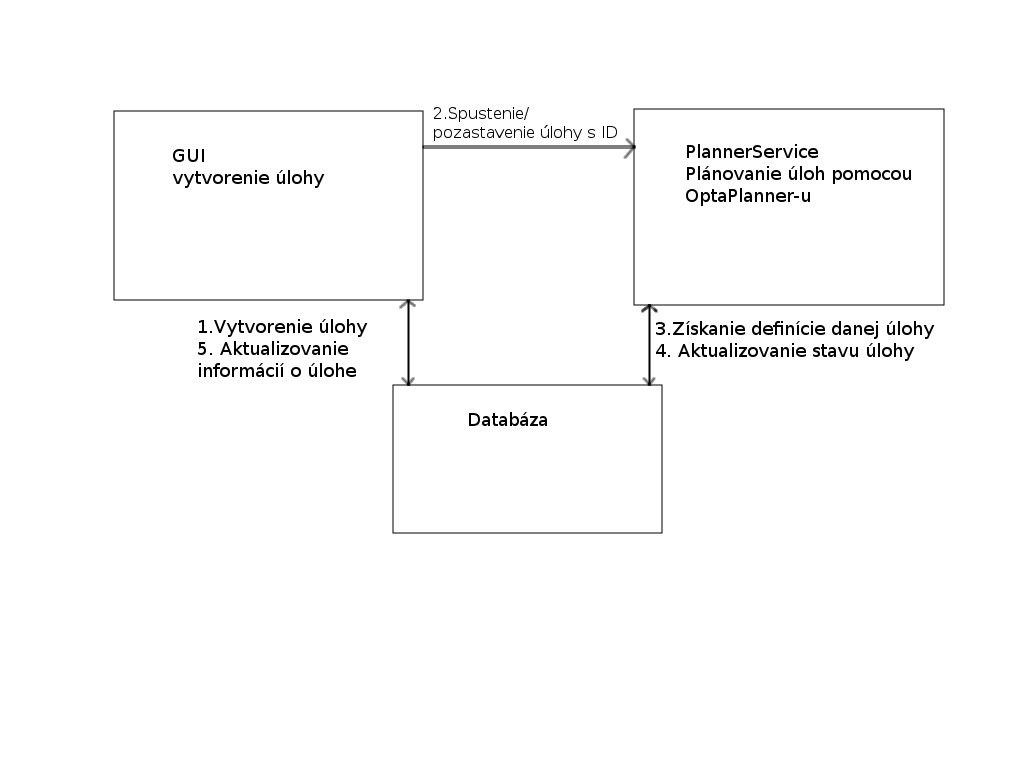
\includegraphics[scale=0.4]{work.jpg} 
\caption{Diagram komunikácie}
\label{work}

\end{center}

\end{figure}
Na obrázku č.\ref{work} je popísané spôsob komunikácie užívateľského rozhrania s PlannerService(OptaPlanner). 1.krokom je vytvorenie XML súboru plánovacieho problému prostredníctvom užívateľského rozhrania a následne uloženie definície do databáze. 2.krok je zaslanie žiadosti s ID úlohy o spustenie/zastavenie prostredníctvom webovej služby PlannerService(OptaPlanner), ktorý žiadosť spracuje. Ten v 3. kroku získa z databáze potrebný definičný XML súbor. Následne sa spustí plánovanie a priebežne sa ukladajú v kroku č. 4 informácie o pokroku úlohy, a čase ukončenia úlohy. Následne užívateľské rozhranie v kroku č. 5 pravidelne získava informácie o úlohe z databáze a zobrazuje ich v prehľadnej tabulke.

Celý návrh aplikácie bol otestovaný prostredníctvom skupiny odborných a laických užívateľov s cieľom zdôrazniť rýchlu učiacu sa krivku užívateľského rozhrania. Následne prebiehalo testovanie prostredníctvom užívateľov, ktorý testovali validáciu vstupov, prihlasovanie, správne vyhľadávanie jednotlivých entít(úloh, užívateĺov, organizácií).

\subsection{Návrh modelu databáze}
Na nasledujúcom obrázku je ukázaný ER diagram, ktorý bol použitý pre dtabázu:
\begin{figure}[htb]

\begin{center}

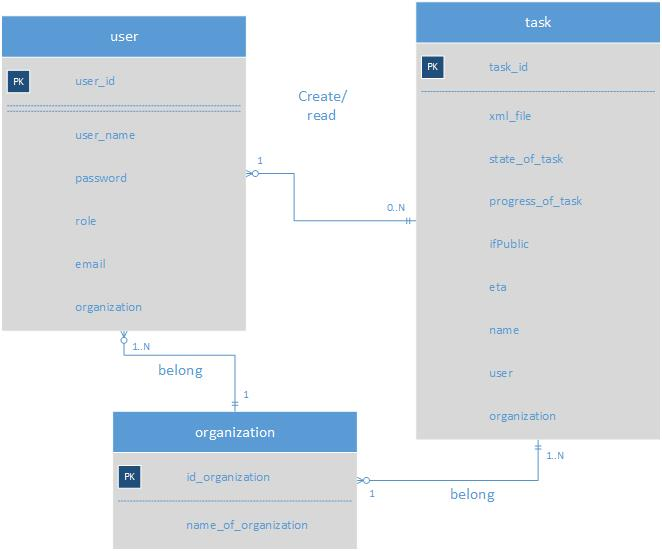
\includegraphics[scale=0.7]{ER.jpg} 
\caption{ER diagram}
\label{ER}

\end{center}

\end{figure}

Tento obrázok zobrazuje jednotlivé entity, ktoré sú potrebné na uloženie v databáze, každá z nich ma určité položky. ER diagram sa skladá z 3 entít: user - entita, ktorá reprezentuje užívateľa, task - entita, ktorá reprezentuje úlohu a organization - entita, ktorá reprezentuje organizáciu. Výsledný návrh odpovedá skutočnosti, že každý užívateľ musí byť súčašťou organizácia, rovnako môže mať vytvorené 0 až N úloh. Taktiež pre zjednodušenie je každa úloha priradená priamo organizácií pre zlepšenie rýchlosti získania výsledkou a zjednodušenia ich nájdenia. Každá entita obsahuje primárny kľúč(jedná sa o silné entitné množiny), ktorý je odvodený od názvu a začína predponou \uv{id\_} a pokračuje názvom entity s CamelCase notáciou(každé slovo začína veľkým písmenom a slová sú spojené dokopy). Poďme sa pozrieť bližšie na jednotlivé entity. Entitná množina organization obsahuje 2 položky jednou z nich je primárny klúč a ďalšou názov organizácia podľa, ktorej sú zaraďovaný jednotlivý užívatelia. Ďalej prejdime k entitnej množine user. Táto entita má rovnako primárny kľúč. Ďalej obsahuje položku pre užívateľské meno(username), heslo(password), email, užívateľskú rolu(role) a cudzí kľúč organization, ktorý obsahuje na odkaz na organizáciu, ku ktorej je užívateľ priradený. Nakoniec prejdime k entitnej množine task. Táto entitná množina obsahuje primárny kľúč, ďalej obsahuje XML súbor, ktorý reprezentuje danú úlohu(v našom prípade N dám), stav úloh(stateOfTask, ktorý reprezentuje rôzne stavy úlohy), ktorý si podrobnejšie rozobereme. Úloha sa môže nachádzať v jednom z nasledujúcich stavov:
\begin{itemize}
\item NEW - úloha bola vytvorená
\item MODIFIED - XML súbor bol modifikovaný
\item WAITING - úloha čaká na spracovanie
\item IN\_PROGRESS - práve prebieha výpočet
\item PAUSED - úloha je pozastavená
\item COMPLETE - úloha je dokončená
\end{itemize}
Entitná množina task ďalej obsahuje položku, ktorá percentuálne hodnotí stav výpočtu úlohy(progressOfTask), čas do skončenia výpočtu úlohy(eta), nastavenie úlohy na privátnu alebo verejnú(ifPublic), názov úlohy(name) a cudzie kľúce user, ktorý odkazuje na užívateľa, ktorým bola úloha vytvorená a organization, ktorá odkazuje na organizáciu užívateľa, ktorým bola vytvorená. 

\subsection{Návrh užívateľského rozhrania}
Výsledné rozhranie kladie dôraz na jednoduchosť a prehľadnosť zobrazených úloh. Z tôhto dôvodu boli implementované mechanizmy vyhľadávanie úloh, organizácií a užívateľov. Rovnako možnosti lexikografického triedenia. Po prihlásení do systému Jednotlivé môžnosti sú následe zakomponované do záložiek, v ktorých je sprístupnená príslušná funkčnosť. Výsledné rozhranie je prenositeľné aj na mobilné zaradenie. Užívateľské rozhranie je popísané na nasledujúcom obrázku:
\begin{figure}[htb]

\begin{center}

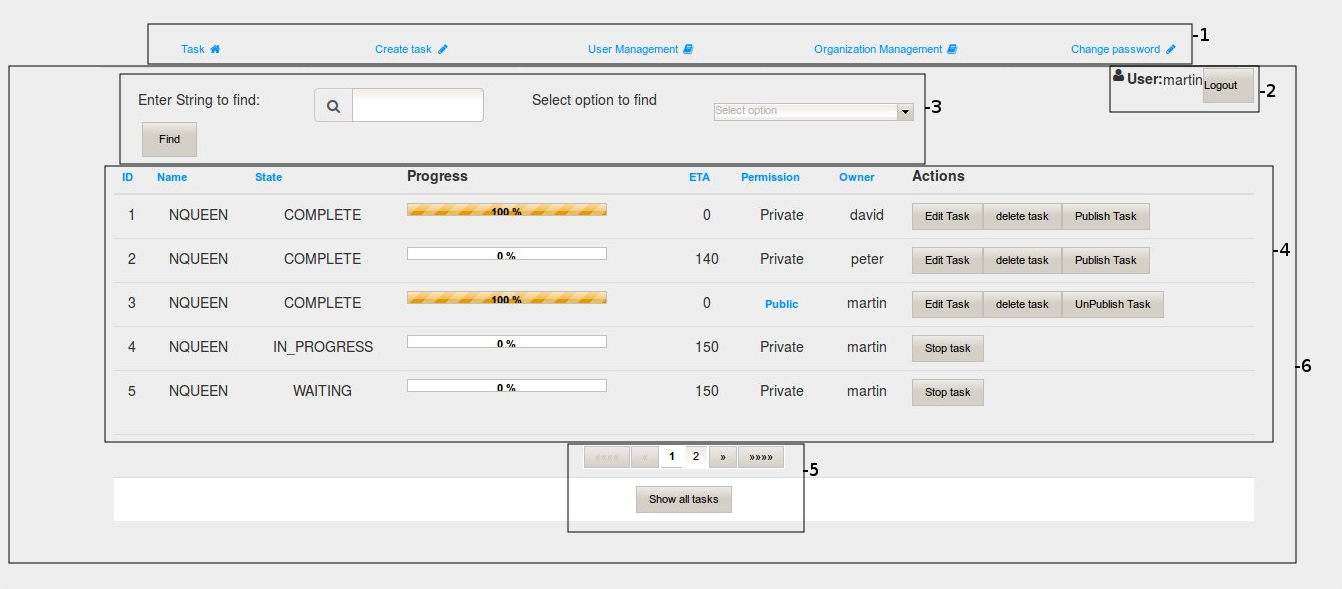
\includegraphics[scale=0.4]{page.jpg} 
\caption{Návrh užívateľského rozhrania}
\label{rozhranie}

\end{center}

\end{figure}
Na obrázku č.\ref{rozhranie} môžme vidieť návrh užívateľského rozhrania. Rozhranie je rozdelené do 6 častí, ktoré môžme rozoznať na obrázku číslami od 1 do 6, ktoré sú aj ohraničené. Celé rozhranie môžme rozdeliť do nasledujúcich častí:
\begin{itemize}
\item Oblasť č.1 predstavuje navigačné menu, kde sú jednotlivé akcie rozdelené do záložiek podľa ich názvu. Pre klinutí na príslušnú záložku sa zmení aj obsah na stránke. 
\item Oblasť č.2 obsahuje informáciu o prihlásenom užívateľovi , rovnako obsahuje aj tlačidlo \uv{Logout}, prostredníctvom ktorého sa môže užívateľ z aplikácie odhlásiť
\item Oblasť č.6 predstavuje funkčnú oblasť. Táto oblasť je špecifická pre každú záložka, ktorá reprezentuje jej obsah. V tej oblasti sú umiestnené typicky obsahy databázových tabuliek, nástroje na vyhľadávanie, rôzne akcie, ktoré je možné vykonávať s dátami, rovnako aj možnosti na vytváranie entít
\item Oblasť č.3 predstavuje jednu z funkčných možností. Jedná sa o vyhľadávanie, ktoré je zložené zo vstupného prvky, do ktorého zadamé vyhľadávaný reťazec a druhá časť predstavuje menu,z ktorého zvolíme stĺpec na vyhľadávanie. Následne je možnosť realizovať tlačidlom Find, ktoré prekreslí obsah tabulky nižšie a naplní ju nájdenými výsledkami.
\item Oblasť č.4 predstavuje tabulky, ktorá je dynamicky obnovaná a reaguje na asychronné ukladanie dát z web service, ktoré sa dynamicky obnovujú každé 4 sekundy. Tabuľka je rozdelená do stĺpcov. Názvy stĺpcov, ktoré sú označené modrou farbou sú zároveň odkazy, na ktoré je možné klinúť. Po kliknutí na daný odkaz dôjde k lexikografickému zoradeniu obsahu tabuľky podla daného stĺpca striedavo vzostupne alebo zostupne. Rád by som upozornil na stĺpec progress, ktorý pre každú úlohu zobrazuje stav spracovania úlohy. Rovnako musím zdôrazniť stĺpec Permission, ktorý zobrazuje, či je úloha verejná alebo privátna. Pokiaľ je úloha verejná(Public), tak je tento odkaz zobrazený modrou farbou, čo znamená, že je odkaz preto je možné naň ho kliknúť. Po kliknutí sa zobrazí stránka s informáciami o názve úlohy a obsahuje výsledného xml súboru. Tento odkaz je možné následne ľubovolne preposlať a pristupovať k nemu. V poslednom rade treba zdôrazniť stĺpec \uv{Actions}, ktorý je najdôležitejší pre každú úlohu povoluje sadu akcií. Jednotlivé akcie sú reprezentované tlačidlami, pritom odrážajú aktuálny stav spracovania úlohy spolu s ďalšími informácimi o úlohe.
\item Oblasť č.5 predstavuje komponentu na stránkovanie, aby pri rozsiahlom obsahu sa nezväčšoval neúmerne veľkosť stránky.


\end{itemize}

Zvyšné návrhy rozhrania pre vytvorenie úlohy, editovanie úlohy, spravovanie užívateľov, spravovanie organizácií, zmenu hesla a prihlasovanie je možné dohľadať v prílohe.


\chapter{Implementácie}\ref{implc}
Nasledujúca kapitola pojedná o oboch častiach systému pre monitorovanie stavu plánovacích úloh.  Najprv rozobereme aplikáciu pre užívateľské rozhranie\ref{approz} a následne PlannerService\ref{plannerapp}, ktorá zabezpečuje riešenie plánovacích úloh prostredníctvom OptaPlanner-u. Pre technológiu MySQL bol zvolený MySQL server vo verzii 5.5.37. Obe časť boli založené na nástroji maven\cite{mavenbook} s použitím vývojové prostredia JBoss Developer Studio vo verzii 7.1.0 GA. 


\section{Aplikácie pre užívateľské rozhranie}\label{approz}
Aplikácie pre užívateľské rozhranie, ktorá je schopná zobrazovať informácie o úlohách, užívateľoch a organizáciach a umožňovať ich správu. Základom tejto aplikácie je komunikácia s databázou. Komunikáciu zabezpečuje JBoss a to tak, že sa v súbore persistence.xml pre našu aplikáciu(\emph{optapanner.controller}) správne nastaví odkaz na datasource a definíciu entitných tried.
	

\subsection{Prihlasovanie}
Prihlasovanie je realizované prostredníctvom frameworku Seam. Základom je vytvorenie komponent na XHTML stránke pre zadanie mena a hesla užívateľa. Tieto údaje sú spracované v backing bean-e(triede) s názvom \emph{LoginBean}, ktorá je súčasťou balíku \emph{org.jboss.optaplanner.controller.beans}. Táto trieda obsahuje aj validátory(metódy validateUsername/validatePassword), ktoré kontrolujú existenciu užívateľa a správnosť hesla v prípade, že existuje a podľa zistených informácií(existuje užívateľ/neexistuje, validné/nevalidné heslo) sa zobrazí komponenta \emph{h:outputText}, ktorá obsahuje príslušný text.

V prípade, že validácia prebehne úspešne zavolá sa metóda \emph{authenticate}, ktorá zabezpečí získanie užívateľskej role zadaného užívateľa, ktorú následne vloží do životného cyklu aplikácie pomocou metódy \emph{setUser}, a to pomocou triedy \emph{org.picketlink.idm.api.User} sa vloží ID užívateľa a užívateľská rola.

Navigácia užívateľa sa realizuje nastavením navigačných pravidiel v súbore \emph{faces-config.xml}, do ktorého sa podľa užívateľske role užívateľa nastaví hodnota premennej isX(Admin/Planner/Reader) na hodnotu TRUE a zabezpečí presmerovanie užívateľa na stránku podľa role:
\begin{itemize}
\item Rola Administrator bude presmerovaná na stránku Administrator.xhtml 
\item Rola Planner bude presmerovaná na stránku Planner.xhtml
\item Rola Reader bude presmerovaná na stránku Reader.xhtml
\end{itemize}

Úspešné prihlásenie je dané nastavení metódy \emph{setStatus} na hodnotu SUCCESS, v prípade, že validácia údajov neprebehne úspešne nastavíme prihlasovanie na neúspešné prostredníctvom metódy \emph{setStatus} na hodnotu FAILURE. Po uspešnom prihlásení je možné identitu ľahko získať nainjektovaním(uvedením anotácie @Inject) triedy Identity, z ktorej je možné získať prihlasovacie meno užívateľa, ktorá sa zobrazuje na stránke.

Problematika odhlasovania úzko súvisí s prihlasovaním a je v podstate jednoduchá. Na XHTML stránke sa nachádza grafická komponenta \emph{h:commandButton}, ktorá v atribúte action volá metódu logout pre príslušnú backing beanu. Tá spôsobí zavolanie metódy identity.logout, ktorá odobere identitu daného užívateľa(zamedzí mu opätovnú prístup k stránke podľa jeho role) a presmeruje ho na prihlasovacie stránku(Login.xhtml).

\subsection{Zabezpečenie}
Úzko s prihlasovaním súvisí aj prolematika zabezpečenia aplikácie proti neutorizovanému prístupu. Teda povedzme užívateľ s rolou Planner by chcel pristúpiť na stránku, ktorá je určená pre rolu Administrator. Aplikácia mu to nedovolí a v prípade o takýto pokus bude užívateľ presmerovaný naspäť na prihlasovaciu stránku. Princíp je taký nájden rozhranie, ktoré je anotovaná anotáciu @ViewConfig. Táto trieda obsahuje výpočtový typ, ktorý obsahuje anotácie @ViewPattern, ktorej obsah je stránka, na ktorú má byť povolený prístup. Pri každej takej anotácií je nachádza názov užívateľskej role uvedený prostredníctvom anotácie. Použitie názvu užívateľskej role je dané vytvorením špeciálneho rozhrania, ktoré je anotované anotáciu \emph{SecurityBindingType}. Uvedenie anotovanej užívateľskej role vedľa stránky, ktorá má byť povolená spôsobí zavolenie triedy \emph{Autorization}, ktorá je anotovaná anotáciu \emph{Service}, ktorá overí vloženú identitu prostredníctvom metódy \emph{authenticate} z triedy \emph{LoginBean} a vráti odpoveď. Takýmto spôsobom sa povolí prístup pre užívateľskú rolu na danú stránku. Veďla každej anotácie @ViewPattern sa nachádza aj anotácia \emph{AccessDeniedView}, ktorá spôsobí presmerovaní na jej obsah, v prípade, že prihlásený užívateľ nemá danú užívateľskú rolu. Tento postup sa opakuje neustále v prípade pokusu o prístup k akejkoľvek stránke uvedenej rozhraní anotovaní anotáciou \emph{ViewConfig}.



\subsection{Komunikácie s PlannerService}
Základom komunikácie s výpočtou časťou systému PlannerService je vygenerovanie klienta z WSDL súboru webovej služby. Preto bolo potrebné vykonať nasledovné kroky:
\begin{itemize}
\item Nasadenie PlannerService na JBoss
\item Zavolanie skriptu wsconsume.sh, ktorý je súčasťou aplikačného serveru s prepínačom -k a cestou k WSDL súboru
\item Skopírovanie vygenerovaných tried do aplikácie pre užívateľské rozhranie do balíku \emph{org.jboss.optaplanner.controller.service}
\end{itemize}
Po týchto krokoch sa v metóde \emph{runTask} a \emph{stopTask} volá metóda, ktorá vytvorí webovú službu a zavolá metódu runTask/pauseTask, ktoré sú súčasťou PlannerService s argumentom ID úlohy. Tieto metódy sú súčasťou backing bean pre užívateľsku rolu Planner a Administrator.


\subsection{Logika aplikácie}
Pre každú užívateľskú rolu bola vytvorená 1 XHTML stránka a backing beana a to nasledovne:
\begin{itemize}
\item Pre rolu Administrator je určená stránka Administrator.xhtml a backing beana(trieda) \emph{AdministratorBean}
\item Pre rolu Planner je určená stránka Planner.xhtml a backing beana(trieda) \emph{PlannerBean}
\item Pre rolu Reader je určená stránka Reader.xhtml a backing beana(trieda) \emph{ReaderBean}
\end{itemize}
Všetky backing beany sú súčasťou balíka \emph{org.jboss.optaplanner.controller.beans}. Aby beany mohli byť správne používané je potrebné ich uviesť v súbore faces-config.xml. To sa urobí uvedením medzi značky \emph{managed-bean}, kde uvedieme názov beany, triedu vrátane cesty v hierarchii balíkov a typ beany(ktorý bol zvolený na session). Backing bean-y obsahujú metódy a vlastnosti, ktoré bola zobrazované/prevzaté z komponent na .xhtml stránkach. Všetky vlasnosti museli spĺňať princíp POJO. Pre potreby získavania dát z databáze bola použitá trieda \emph{databaseOp}, ktorá je súčasťou balíku \\\emph{org.jboss.optaplanner.controller.database}, pričom vytvára inštanciu triedy EntityManager, ktorý využíva entitné triedy. Táto trieda obsahuje metódy na vytváranie úloh, užívateľov, organizácií, rovnako aj mazanie, editovanie jednotlivých položiek, rovnako aj získavanie. Tieto dáta sú následne predávané backing bean-ám podľa potreby.


\subsection{Implementácia rozhrania}
Pre implementáciu rozhrania bola použitá technológia XHTML stránok. Pre každú užívateľskú rolu bola vytvorená XHTML stránku identitická s názvom užívateľskej role. Pre prihlasovanie bola použitá  stránka Login.xhtml stránka. Na Login.xhtml boli umiestnené komponenty na zadanie užívateľského mena a hesla vrátane skrytých validačných komponent. Na tejto stránke boli použité správne CSS frameworky na zabezpečenie prenositeľnosti na mobilné zariadenia a zároveň poskytli užívateľskú prívetivosť.

Pri implementáciu XHTML stránok pre užívateľské role sa zameriam na užívateľskú rolu Administrátor, keďže rola Plánovač a Čitateľ prevzali všetku implementáciu a komponenty práve od Administrátor, ale len v obmedzenom množstve, teda komponenty vrátane akcií, ktoré mohli vykonávať. XHTML stránka sa skladá v hornej časti z menu, ktoré je implementované ako záložky. V pravej hornej časti sa nachádza informácia o prihlásenom užívatelovi vrátane tlačidla na odhlásenie.  


Pri kliknutí na záložky sa zobrazí obsah, ktorý odpovedá názvu záložku. Záložky \uv{user management, task, organization management} obsahujú komponenty h:datatable z knižnice JSF pre zobrazenie dát. Tieto dáta sú pravidelné obnovované z databáze, čo zabezpečuje ich aktuálnosť prostredníctvom komponenty a4j:poll, ktorá je vytvorená pre každú tabuľku a pravidelne volá metódu, ktorá získava údaje z databáze. Každá z tých záložiek obsahuje pole pre vyhľadávanie, pričom je možné zvoliť podľa, ktorého stĺpca sa bude vyhľadávať. Výsledky sa zobrazia do tabuľky(h:datatable) pričom zobrazené položky budú odpovedať nájdeným výsledkom. Pri vyhľadávaní sa prerušení obnovanie obsahu tabuliek a zobrazí sa informácie o vyhľadávanom reťazci a časovom razítku kedy bolo vyhľadávanie realizované. S vyhľadanými položkami je rovnako možné realizovať všetky akcie. Pre potreby opätovného obnovenia obsahu tabuľky je potrebné stlačiť tlačidlo pod tabuľkou s názvom \emph{showX(Users,Tasks,Organizations)}, ktoré sa nachádza na bielom páse pre rýchlejšie zorientovanie užívateľa. Toto tlačidlo spôsobí pre danú tabuľku(users,taks,organizations) získanie aktuálnych dát z databáze zavolaním metódy z triedy \emph{databaseOp} getAllX(Tasks/Users/Organizations), ktoré vytvoria dotaz na získanie aktuálnych dát z databáze. Tieto dáta sú predané príslušnej tabuľke a zároveň sa obnoví obnovovanie obsahu tabuliek.

 Pri každej položke v tabuľke je možné vykonávať isté akcie ako je vymazať danú entitu(task,user,organization), po prípade ju editovať, alebo vykonávať množstvo iných akcií. Akcie pritom reflektujú individuálny stav danej entity. Pri každej z tých záložiek okrem task(ktorú v zápäti rozoberem) je možné entity aj vytvárať. Vytváranie je veľmi jednoduché, keď užívateľ vyplní všetky polia, ktoré musí mať daná entita sa zavolá metódu z backing beany(napr. na editovanie editTask, na vytvorenie organizácie createOrganization, \ldots), ktoré spôsobia zavolanie metódy z triedy \emph{databaseOp}, ktoré zabezpečia vytvorenie novej entity. 

 Každú tabuľke je možné aj radiť. Radenie prebieha kliknutím na názov stĺpca tabuľky(zvýraznený modrou farbou), pričom danú stĺpec implementuje funkciu radenia pre daný stĺpec. Pri kliknutí na názov stĺpca dôjde k zavolanie metódy(napr. pre stĺpec ID sa zavolá metóda sortById), ktorá je daná atribútom action v grafickej komponente \emph{h:commandLink}. Metóda radenia je implementovaná prostredníctvom triedy \emph{Collections}, ktorá obsahuje metódu sort, ktoré triedia model(trieda, ktorá obsahuje rovnaké položky ako príslušna databázová tabuľka) danej entity, ktorá vytvorí komparátor, ktorý porovná 2 položky daného modelu a upraví ich poradie.


Vytváranie úloh(taskov) je zaradené do samostatnej záložky kvôli lepšej prehľadnosti. Užívateľ vyplní názov a prostredníctvom komponenty na nahrávanie súboru z knižnice Rich Faces nahrá obsah do databáze. Ďalej rozoberem záložku change password, ktorá umožňuje si pre daného užívateľa zmeniť heslo, vyplní pritom heslo a potvrdenie heslo a heslo sa zmení. Nakoniec rozoberem záložku edittask, táto záložka je pri bežnom prehliadaní nevidelná je to spravené kvôli bezpečnosti. Táto záložka sa aktivuje editovaním úlohy v záložke task v tabuľke tlačidlom Edit Task, ktorá nás prepne do záložky Edit Task, v ktorej sa už aktivuje obsah a užívateľ vyplní názov úlohy,vlastníka úlohy a nakoniec edituje xml súbor úlohy. Potvrdením sa vytvorí úloha so stavom \uv{MODIFIED}.


\subsection{Publikovanie úloh}
Ďalšou podstatnou časťou aplikácie pre užívateľské rozhranie je možnosť publikovať/odpublikovať úlohu(task). Túto akciu je možné realizovať prostredníctvom tlačidla v tabuľke Publish Task/Unpublish Task. Tieto tlačidlá nie sú vždy prístupné, podmienkou je, že úloha je nastavená ako privátna a nachádza v stave \uv{MODIFIED} alebo \uv{COMPLETE}. Naopak odpublikovanie úlohy je možné kedykoľvek podmienkou je, aby úloha bola nastavená ako verejná(public). Publikovanie je realizovaná zavolaním metódy \uv{publishTask}. V tejto metóde dôjde k zmene stavu úlohy na verejenú, pričom informácia sa uloží do databáze. Následne sa v stĺpci permission zobrazí text \emph{Public} modrou farbou, ktorý po kliknutí zobrazí názov úlohy a XML súbor plánovacej úlohy. Pričom po kliknutí sa prejde na odkaz \emph{url aplikácie/task/id úlohy}. Na časť URL task/id je namapovaná rest webová služba, ktorá je súčasťou balíku \emph{org.jboss.optaplanner.controller.restservice}, kde sa nachádza trieda \emph{RESTPublishTask}, ktorá reprezentuje práve túto službu starajúcu sa o publikovanie úloh. Táto úloha obsahuje v anotácií @Path() len znak \uv{/},čo znamená že sa namapuje na akékoľvek URL, ale namapovanie na reťazec task sa realizuje v súbore web.xml. Táto služba obsahuje 1 metóda \uv{getUserById}, ktorá dostane ako parameter ID úlohy. Toto id úlohy získa zo zadaného URL. Dôležitou anotáciu je anotácia @Produces(), ktorá obsahuje hodnotu \uv{text/html}, ktorá hovorí, že vrátená odpoveď metódy bude HTML súbor a teda výsledok bude zobrazený v prehliadači. Táto metóda na svojom začiatku vytiahne informácie o úlohe(názov, XML súbor a povolenie). Na základe povolenia určí, či je úloha nastavená ako verejná, ak nie je vráti prázdnu stránku. V prípade, že je úloha verejná vráti stránku, ktorá obsahuje informáciu o názvu úlohy a XML súbor. Prístup k tomuto k tejto službe nie je podmienený prihlasovaním.


\subsection{Validácia}
Všetky grafické komponenty obsahujú validáciu na neprázdne, niektoré aj na nevalidné komponenty. Všetky komponenty, do ktorých sa zadáva nejaká informácia je realizovaná grafickou komponentou \emph{h:inputText}, ktoré spracovávajú užívateľské vstupy. Každá komponenta obsahuje atribút \emph{required} nastavenú na hodnotu true, ktorá spôsobí automatickú validáciu v prípade nezadanej hodnoty. Každá komponenta obsahuje aj atribút \emph{requiredMessage}, ktorý ako hodnotu obsahuje reťazec, ktorý sa zobrazí v prípade, že nie je zadaná hodnota. Rovnako obsahuje aj atribút ID s nejakou jedinečnou hodnotou pre identifikáciu komponenty. Aby informácia o nezadaní bola zobrazená je potrebné vytvoriť komponentu h:message, ktorá obsahuje atribút for, ktorý obsahuje id h:inputText komponenty, pre ktorú má byť správa zobrazená. Niektoré komponenty(napr. validácia prihlásenia) sú validované na základe validátorov, ktoré obsahujú odkaz na metódy v triede \emph{LoginBean}, ktoré v prípade potreby nastavia zobrazenie komponenty h:outputText prostredníctvom nastavenia atribútu rendered na hodnotu true, pričom táto komponenta obsahuje text podľa danej situácie(napr. neznámy užívateľ, nevalidné heslo). V opačnom prípade je komponenta skrytá, teda hodnota atribútu je nastavená na hodnotu false.




\section{PlannerService}\label{plannerapp}
PlannerService predstavuje časť systému pre monitorovania, ktorá zabezpečuje spracovanie požiadavok od aplikácie z užívateľského rozhrania. Základom je trieda \emph{OptaPlanerWebService}, ktorá predstavuje \uv{Big} webovú službu, ktorá je súčasťou balíku \\\emph{org.jboss.optaplanner.service.server}. Tá je špeciálne anotovaná prostredníctvom anotácie @WebService, ktorá označuje, že daná trieda je webovou službou. Tá obsahuje 2 metódy \uv{runTask} a \uv{pauseTask}, ktoré sú anotované anotácou @WebMethod, a sú teda prístupne a môžu byť vzdialene zavolané klientom(aplikáciou pre užívateľské rozhranie). Ako argument obsahujú metódy hodnotu typu long, ktorá predstavuje ID plánovacej úlohy, s ktorou sa má daná akcia vykonať.

Druhou dôležitou triedou je \emph{OptaPlannerMessageBean}, ktorá je súčaštou balíku \\\emph{org.jboss.optaplanner.service.server}. Táto trieda predstavuje Message-driven bean-u a je anotovaná anotáciu @MessageDriven a pre prijímanie požiadavkov využíva JMS frontu s názvom \emph{OptaPlanner}.

Základným predpokladom je korektné nastavenie súboru persitence.xml, ktorý odkazuje na entitné triedy a odkaz na datasource.

Princíp fungovania tejto časti systému je nasledujúca:
\begin{itemize}
\item Klient(aplikácia užívateľského rozhrania) zadá požiadavok na spustenie/pozastavenie úlohy, ktorú realizuje zavolaním metódy webovej služny PlannerService s ID plánovacej úlohy
\item Metóda runTask PlannerService vytvorí spojenie s triedou \emph{OptaPlannerMessageBean}, a následne vložením správy s ID úlohy do JMS fronty \emph{OptaPlanner}
\item Trieda \emph{OptaPlannerMessageBean}, ktorá je Message-driven bean tá obsahuje odkaz rovnako na JMS frontu \emph{OptaPlanner}. Tá obsahuje metódu \emph{onMessage}, ktorá zabezpečuje spracovánie správ z JMS fronty \emph{OptaPlanner} správu po správe
\item Metóda \emph{onMessage} získa zo správy ID úlohy, ktorú následne získa z databáze, zmení stav úlohy na \emph{IN\_PROGRESS} a vytvorí inštanciu triedy \emph{ProblemSolver}, ktorej konštruktor dostane ako parameter XML súbor plánovacej úlohy z databáze. Táto trieda je súčaštou balíku \\\emph{org.jboss.optaplanner.service.solver}. Po vykonaní tohto kroku sa spustí metóda \emph{run}, ktorá nastaví konfiguráciu pre riešenie problému N Dám. Následne sa zavolá metóda \emph{execute}, ktorá spustí výpočet(riešenie).
\item V message-driven bean sa v cykle neustále získava skóre z triedy \emph{ProblemSolver} na základe, ktorého sa počítajú hodnoty do času skončenia úlohy a pokroku, ktoré sa zapisujú do databáze.
\item Po ukončení/vyriešení úlohy sa z triedy \emph{ProblemSolver} získa najlepšie riešenie(XML predpis), ktorý sa uloží do databáze s informáciami o dokončení úlohy(zmení stav úlohy na \emph{COMPLETE})
\item Tento postup sa opakuje pre všetky správy v JMS fronte \emph{OptaPlanner}
\end{itemize}

Na koniec spomeniem princíp fungovania metódy na pozastavenie vykonávania plánovania:
\begin{itemize}
\item Klient(aplikácie užívateľského rozhrania) zavolá metódu \emph{pauseTask} s argumentom ID úlohy, ktorá sa má pozastaviť
\item Metóda \emph{pauseTask} triedy \emph{OptaPlannerWebService} spôsobí zmenu stav úlohu na \emph{PAUSE}
\item Message-driven bean v metóde \emph{onMessage} neustále obnovuje hodnoty o priebehu vykonávaní funkcie a podmienke cyklu je podmienka,že úloha je nastavená na stav \emph{IN\_PROGRESS}. Teda v prípade zmeny stavu sa cyklus zastaví a teda aj výpočet(riešenie)
\end{itemize}
	
	



 
\section{Testovanie}
Testovanie prebiehalo na servery JBoss AS 7.1.1 Final najprv prostredníctvom jednodúch JUnit testov, ktoré malo overiť komplikovanú fukčnosť metód. Následne sa pre overenie fukčnosti databáze použil framework Arqullian, ktorý umožňuje nasadenie tried priamo do Java EE kontajneru, čo zjednodušuje testovanie. Prostredníctvom tohto frameworku sa testovala celková fukčnosť aplikácie. Jednoduchšie časti boli otestované pomocou JUnit testov. Postupným budovaním aplikácie sa pristupovalo k testovaniu navrhnutých častí. Junit boli postupne skonštruované pre jednoduchšie metódy, ako je overenie funkčnosti vyhľadávania entít, mazanie entít, pridanie entít do zoznamu úloh. 


V ďalšej častie prebiehalo testovanie medzi konkrétnymi užívateľmi. Išlo o 4 informaticky skúsených užívateľov a 4 laikov. Užívatelia testovali celkovú funkčnosť aplikácie a hľadali prípadné chyby, ktoré neodhalilo predošlé testovanie. Aplikácia bola vložená na cloudovú službu OpenShift, ktorá umožnila prístup k aplikácií prostredníctvom internetu. Následne bol skupine užívateľov predložený odkaz na nasadenú aplikáciu a prihlasovacie údaje k užívateľovi s rolou Administrator,Planner a Reader. 

Užívatelia nasledne testovali vytváranie užívatelov, organizácií, úloh. Následne mohli sledovať stav spracovania plánovacich úloh. Aplikáciu otestovali pod 2 prehliadačmi a to Google Chrome vo verzii 34.0 a Mozilla Firefox verzie 28.0. Bol použitý operačný systém linux 3.13.0-24-generic s operačným systémom Kubuntu 14.04.Aplikácia sa správala pod obomi rovnako a korektne. Po odhalení chýb boli chyby ohlásené a odstránené a aplikácia bola následne opäť nasadená. Tento postup sa opakoval až dokým neboli odhalené všetky chyby. Na záver zhrniem testy, ktoré boli užívateľmi realizované:
\begin{itemize}
\item Overenie funkčnosti prihlasovania s validnými/nevalidnými údajmi
\item Overenie fukčnosti záložky task(úloh) - mazanie úloh, editovanie úloh, vyhľadávanie úloh vrátanie validácie, publikovanie/odpublikovanie úloh, navigácia medzi stránkami úloh tabuľky, pri editovaní úlohy sa overovalo skrytie záložky edit task pri kliknutí na inú záložku, radenie úloh podľa všetkých stĺpcov
\item Overovanie fukčnosti záložky user(užívateľ) - vytváranie nového užívateľa s validnými/nevalidnými údajmi, vyhľadávanie užívatelov vrátanie zadania nevalidaných údajov, mazanie užívateľov, editovanie informácií o užívateľoch, zmena hesla užívateľovi
\item Overenie funkčnosti záložky organization(organizácia) - vytváranie organizácie, vrátane vyhľadávania s validnými/nevalidnými údajmi, radenie organizácii, mazanie organizácií, editovanie názvu organizácie
\item Overenie funkčnosti záložky changepassword(zmena hesla) - zmenu hesla s validnými/nevalidnými údajmi pre aktuálne prihláseného užívateľa
\item Testovanie užívateľskej prívetivosti rozhrania skúsenými a laickými užívateľmi, rovnako otestovanie užívateľského rozhrania na mobilnom telefóne
\end{itemize}

Rovnako boli užívateľom predložené XML súboru pre riešenie problému N Dám v rozložení pri 4,8,16 dám. Užívatelia nahrali tieto súbory do systému a sledovali priebeh riešenia plánovacieho problému prostredníctvom PlannerService.

Užívateľské rozhranie bolo otestované pre mobilné telefóny na zariadení HUAWEI Honour 2 s prehliadačom Mozzila Firefox, v ktorom sa zobrazovalo korektne.



\section{Vyhodnotenie aplikácie}
Po testovacej fáze nasledovala fáza vyhodnotenia aplikácie. Cieľovej skupine bol po opravení chýb aplikácie predložený dotazník, do ktoréh výplňami rôzne informácie, kde dávali spätnú väzby, chyby v návrhu, rovnako aj v intuitívnosti ovládania. Cieľovou skupinou aplikácie sú užívatelia bez akejkoľvek predchádzajúcej skúsenosti s touto aplikáciou s vekým rozsahom medzi 20 - 40 rokov. Preto bola aplikácia predložená najprv užívateľom skúseným, ktorým bol poskytnutý predchádzajúci styk s aplikáciou a lacikým užívateľom, ktorý nemali žiadny predchádzajúci styk. Výsledkom zistenia, rovnako vyplyvajúce z výsledkou dotazníka je že užívateľské rozhrania až na niektoré časti je veľmi intuitívne. Užívatelia sa ihneď vedeli zorientovať a vykonať danú akciu, vytvoriť užívatela, organizáciu, úlohu. Problém na, ktorý narazili bolo zorientovať pri vyhľadávaní úloh/užívateľov/organizácií a nájsť tlačidlo pod tabuľkou  a obnoviť všetky údaje v tabuľke. Rovnako oceňovali možnosť zobrazovanie tlačidla \emph{Save Changes} pri editovaní tabuľky vedľa položky, ktorá je práve editovaná v danom riadku. Pri vyhľadávaní ocenili užívatelia zachovania zadaných informácií pre vyhľadávanie. V záložke user management(správa užívateľov) navrhovalo presunutie tabuľky s užívateľmi na začiatok, keďže sa nachádzala na neprehľadnom mieste. Užívatelia ocenili možnosť radenia tabuliek po kliknutí na daný stĺpec aj spôsob realizácie. Užívatelia by ocenili pri úlohách mať možnosť informácie o časovom razítku vytvorení úlohy. Prehliadania pomocou tabuliek im prišlo ako veľmi vhodné rovnako aj použitie stránkovania. Užívateľom chýbala možnosť vyhľadávať poďla viacerých kritérií.



Aplíkácia by mohla byť upravená do užívateľsky prívetivejšieho rozhrania a mohli byť zahrnuté všetky názory užívateľov. Rovnako by PlannerService mohla byť rožšírená o spracovanie aj iných typov plánovacích úloh, minimálne tie, ktoré sú podporované štandardnou implementáciou frameworku OptaPlanner, napr. plánovanie práce, problém obchodného cestujúceho, \ldots.


\chapter{Záver}\label{zaver}
Plánovanie s ním spojené problémy narážame v bežnom živote čoraz častejšia. Ešte väčšie problémy tohto typu majú organizácie, ktoré musia dennodenne riešiť ako naplánovať efektívnu prácu svojich zamestnancov, ako správne komunikovať so zákazníkom a mnoho iných problémov. Riešenie klasickým prístupom a to využitím ľudskými zdrojmi je časovo neefektívne, rovnako treba brať do úvahy ľudský faktor. Preto vzniklo riešenie, ktoré odbremeňuje organizácie od riešení komplikovaých plánovacích úloh. Taký software je šírený pod licenciou open-source a nazýva sa Optaplanner. Tento systém je následne možné využívať pre akúkoľvek oblasť plánovania, aká len nás napadne. Jediné obmedzenie tohto systému sú použité plánovacie algoritmy kobinovaný s rôznymi heurestikami. Užívateľ je schopný definovať definíciu problému, pričom sa môžme inšpirovať verejne dostupnými príkladmi, vytvoriť si pravidlá a nechať systém nech nájde optimálne riešenie pre daný problém. Vytvorená aplikácia predstavuje jedným zo spôsobov ako daný systém využiť pre plánovanie. Aplikácia je intuitívna, formálne spĺňa požiadavky, rovnako sú predstavené možnosti rožširenia rozhrania a urobenie tohto rozhrania oveľa užívateľsky prívetivejšie a efektívnejšie.  Rovnako ukazuje akým spôsobom bol systém navrhnutý z implementačného hľadiska, sú vysvetlené technológie potrebné pre implementácui so zreteľom na výhody použitia. Pre systém bol použitý aplikačný server JBoss, ktorý predstavoval medzi dostupnými riešenia najvhodnejší java EE kontajner vzhľadom na použité technológie. Pre lepší návrh by mohla byť aplikácia rozšírená na použitie ich iných plánovacích úloh, rovnako môže byť užívateľské rozhranie rozdelené do viacerých samostatných sekcií kvôli lepšej prehľadnosti. V poslednom rade kvôli lepšej pochopiteľnosti aplikácie by mohla byť aplikácia pre užívateľské rozhranie rozdelená do viacerých balíkov.


 % viz. obsah.tex

  % Pouzita literatura
  % ----------------------------------------------
\ifczech
  \bibliographystyle{czechiso}
\else 
  \bibliographystyle{plain}
%  \bibliographystyle{alpha}
\fi
  \begin{flushleft}
  \bibliography{literatura} % viz. literatura.bib
  \end{flushleft}
  \appendix
  
  %\chapter{Obsah CD}
%\chapter{Manual}
%\chapter{Konfigra�n� soubor}
%\chapter{RelaxNG Sch�ma konfigura�n�ho soboru}
%\chapter{Plakat}

 % viz. prilohy.tex
\end{document}
